\documentclass[11pt]{article}

\usepackage[english]{babel}
\usepackage[dvips]{graphicx}
\usepackage[dvips]{color}
\usepackage{fancyhdr}
\usepackage[small,isu]{caption}
\usepackage{ifthen}
\usepackage{dcolumn}
\usepackage{appendix}
\usepackage{amsmath, amsthm, amssymb}
\usepackage{bm}
\usepackage{subfigure}
\usepackage{textcomp}
\usepackage{hyperref}
\usepackage{pifont}

%\usepackage{amsfonts}
\usepackage{bbold}
%\usepackage{dsfont}
%\usepackage{epsfig}


%\usepackage{braket}
%\usepackage{widetext}
%\usepackage{hyperref}

\newcommand{\vect}[1]{\mathbf{#1}}
\providecommand{\abs}[1]{\lvert#1\rvert}
\providecommand{\evalat}[1]{\biggl.#1\biggr|}
\newcommand{\arctanh}[1]{\operatorname{arctan}}


\setlength{\topmargin}{-1.5cm}
\setlength{\evensidemargin}{-1.0cm}
\setlength{\oddsidemargin}{0.2cm}
\setlength{\textwidth}{15.90cm}
\setlength{\textheight}{21.8cm}


%\pagenumbering{roman}

\begin{document}


%\newcommand{\inputflag}[2]{\mathbf{#1}}
\newcommand{\inputflag}[4]{
\noindent
{\bf #1} ({\textit{#2}}):\\
\begin{tabular}{p{0.3cm}p{15.0cm}}
 &#3\\
\\
 &\textit{Default value}: #4\\
\end{tabular}
\vspace{0.4cm}
}

\newcommand{\filedescription}[2]{
{
\noindent
\filestyle{#1}}:\\
\begin{tabular}{p{0.2cm}p{15.0cm}}
 &#2
\end{tabular}
\vspace{0.4cm}
}
\newcommand{\filestyle}[1]{{\ttfamily #1}}

\pagestyle{empty}
\begin{center}
{\huge U\LARGE{SER'S} \huge G\LARGE{UIDE}}\\
\vspace{3.3cm}
{\Huge \bf SMEAGOL (version 1.2)}\\
\vspace{3.3cm}
\centerline{\large \today}
\vspace{3.3cm}
{{\large Alexandre Reily Rocha, Ivan Rungger and Stefano Sanvito}\\
\textit{School of Physics, Trinity College Dublin, IRELAND}}\\
\vspace{1cm}
{{\large Victor Manuel Garcia Suarez and Jaime Ferrer Rodriguez}\\
\textit{Departamento de Fisica, Universidad de Oviedo, SPAIN}}\\
\vspace{1cm}
{{\large Steve Bailey and Colin J. Lambert}\\
\textit{Department of Physics, Lancaster University, Lancaster, LA14YB, UK}}\\

\vspace{3cm}
\bf smeagol@tcd.ie\\
http://www.smegol.tcd.ie

\end{center}

% Empty Page

\newpage

\pagestyle{plain}
\tableofcontents
\newpage

\section{Introduction}
This is a comprehensive user guide to the quantum electronic transport code SMEAGOL (Spin and Molecular Electronics Algorithm on a Generalized atomic Orbital Landscape) [1, 2].  SMEAGOL is based on the non-equilibrium Green's function (NEGF) formalism for one-particle Hamiltonian. In its present form it uses density functional theory (DFT) with the numerical implementation contained in the code SIESTA [3, 4]. However, SMEAGOL's computational scheme is very general and can be implemented together with any electronic structure methods based on localized basis sets. Alternative implementations are currently under investigation.

In the next sections we will explain how to set up a typical calculation and we will describe the various options. The reader of this user guide is supposed to have familiarity with the non-equilibrium Green's function formalism [5, 6, 7, 8, 9, 10, 11, 12] and with density functional theory [13]. In addition a good knowledge of SIESTA and the SIESTA's input files is necessary since only the SMEAGOL's commands are described here, although a complete input file needs the setting of flags proper of SIESTA. For these we refer to the SIESTA user guide [4].  

\section{The system setup}
%*****************************************************************
\begin{figure}[h]
\center
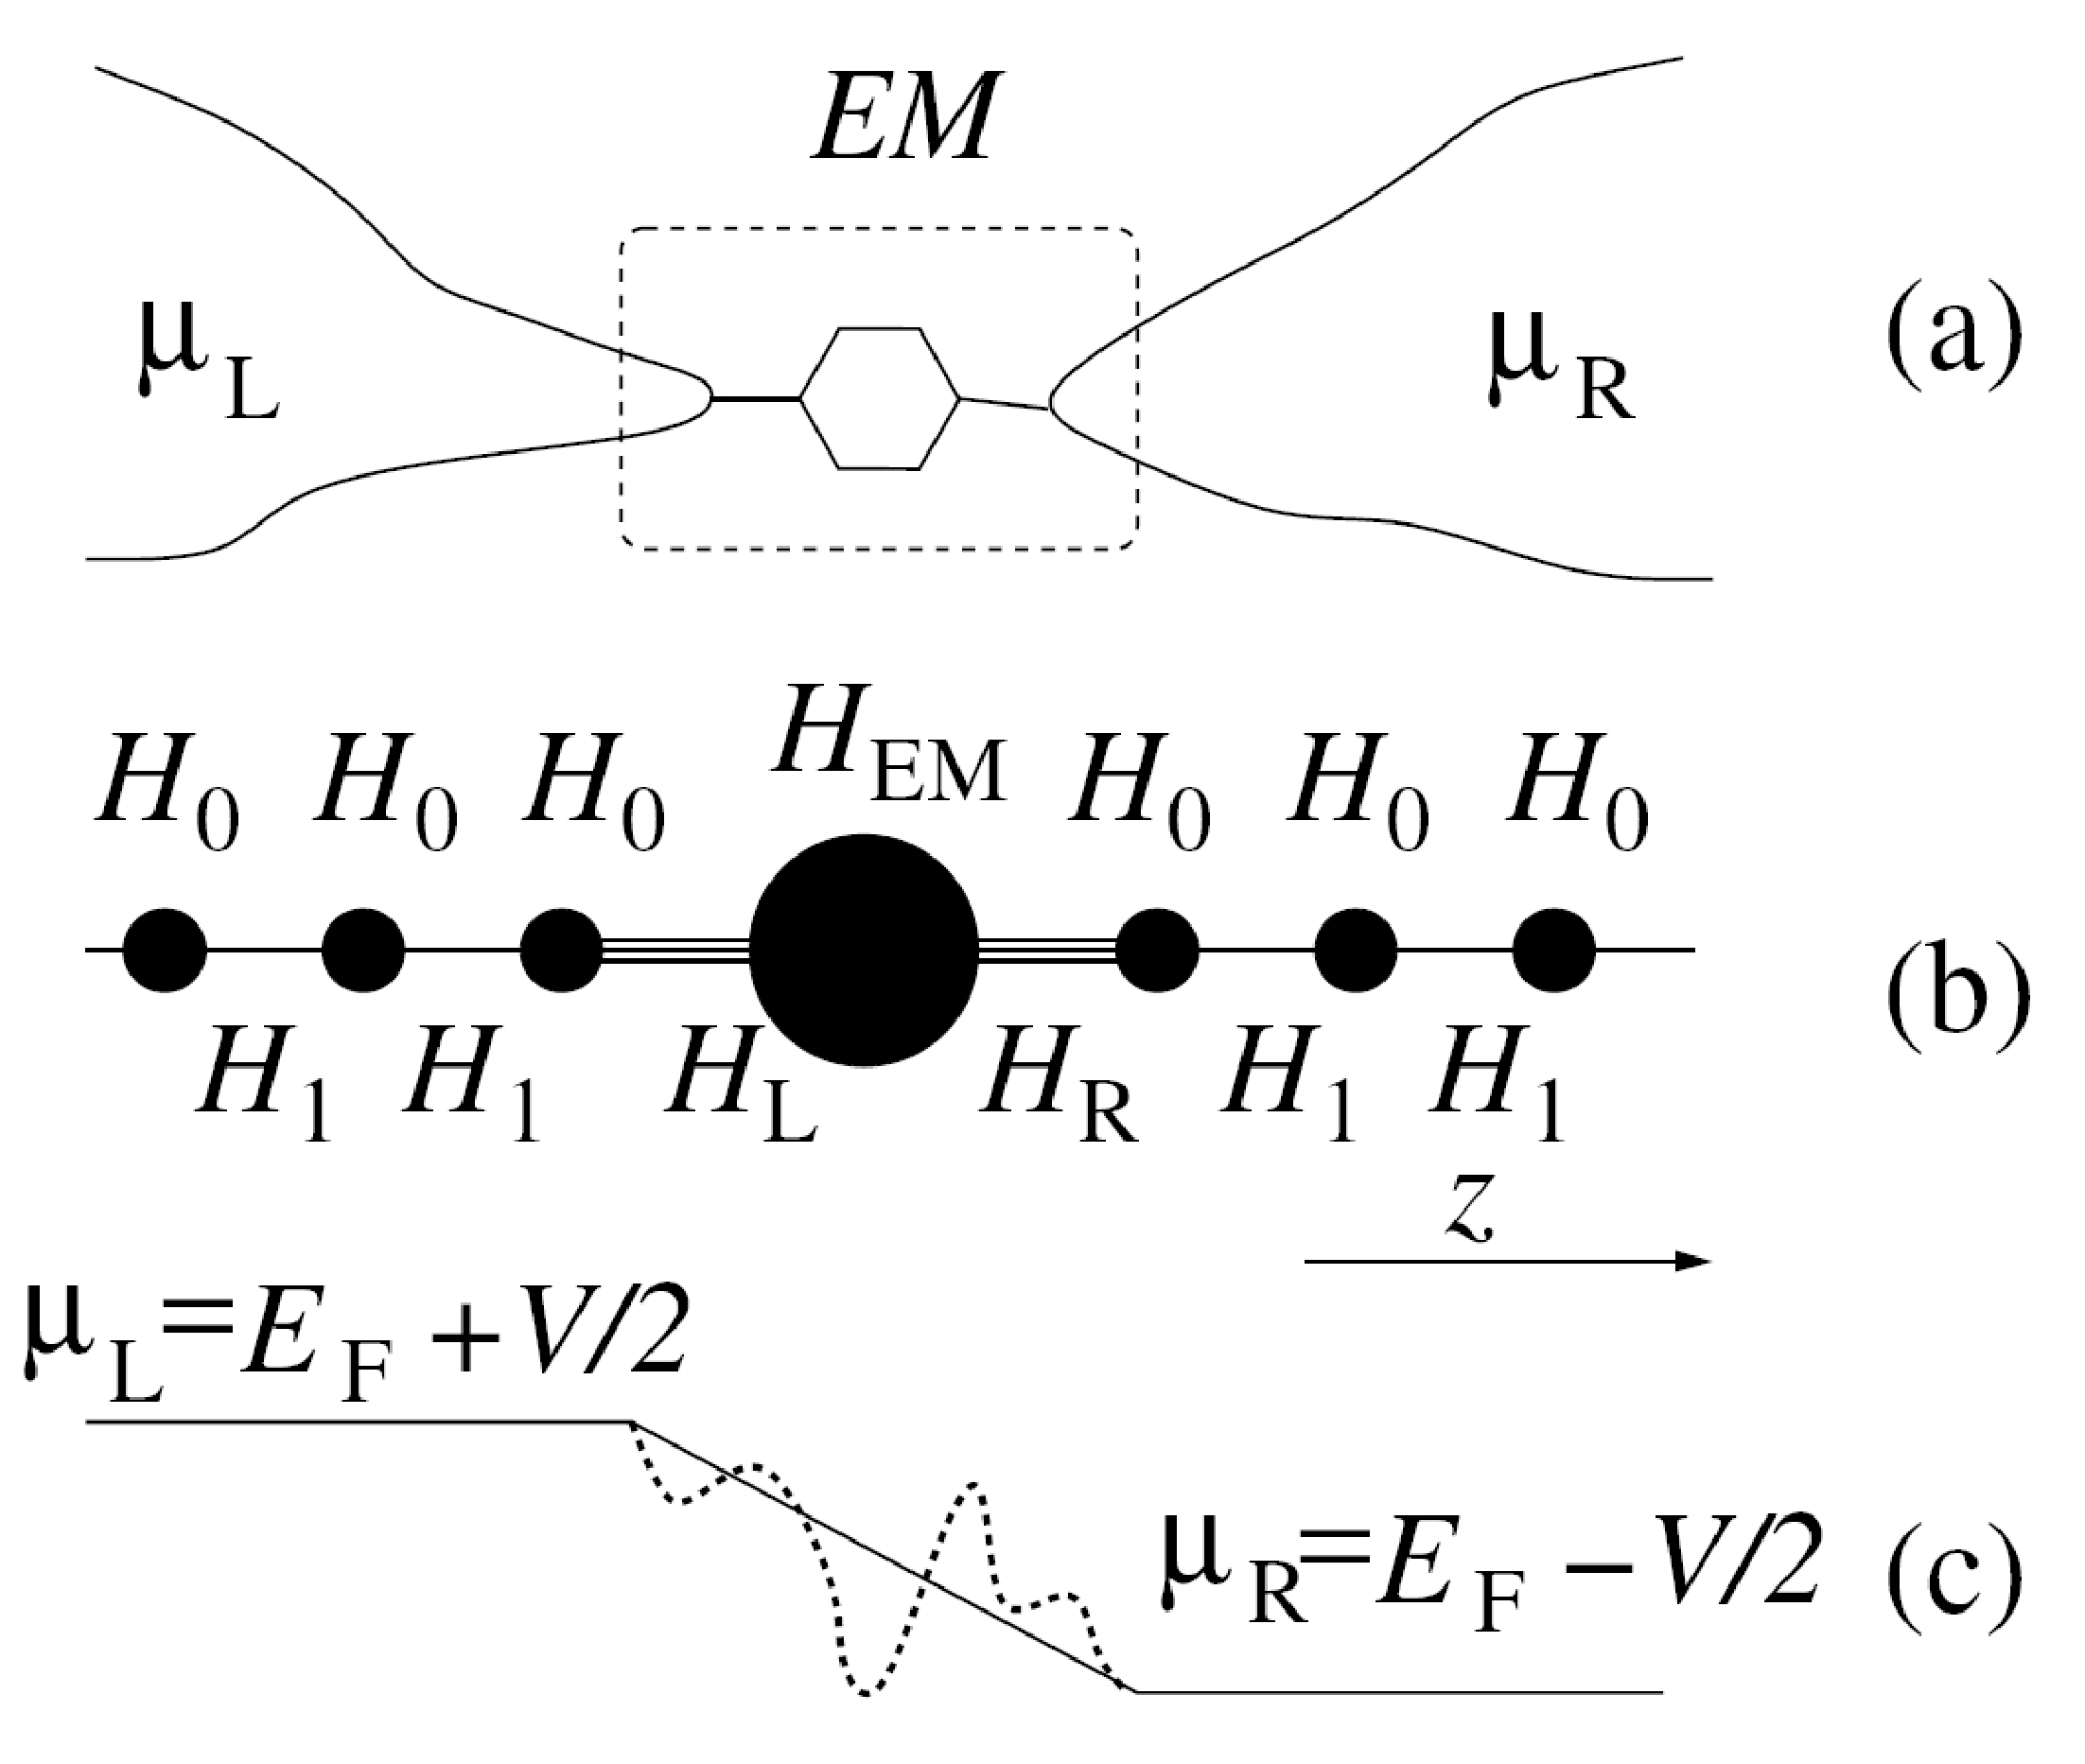
\includegraphics[width=7.5cm,clip=true]{fig/Fig1}
\caption{ (a) Schematic two terminal device. Two leads are kept at the chemical potentials $\mu_L$ and $\mu_R$ and the transport is through the extended molecule (EM). (b) The Hamiltonian is an infinite matrix
comprising two block diagonal parts describing the leads and a part (finite) describing the extended
molecule HEM. (c) Typical potential profile.}
\label{fig:emschem}
\end{figure}
%*****************************************************************


SMEAGOL is designed for calculating two probe $I$-$V$ characteristics. The typical system investigated is described in figure 1. It comprises two semi-infinite leads (left and right) and an extended molecule, which includes the region of interest and a few atomic layers of the leads.  The electronic structure of the leads is not affected by the potential drop and it is computed only once at the beginning of the calculation.

There are two fundamental steps in setting up a SMEAGOL's calculation: 1) calculating the electronic structure for the leads, and 2) calculating the $I$-$V$ curve for a given system. The evaluation of the electronic structure of the leads is essential and must be performed before attempting the calculation of the $I$-$V$ . The files: \filestyle{Systemlabel.HST}, \filestyle{Systemlabel.DM}, \filestyle{bulklft.DAT} and \filestyle{bulkrgt.DAT} are generated during the evaluation of the electronic structure of the leads. These are necessary for calculating the $I$-$V$ characteristic.

\section{The leads calculation}
%*****************************************************************
\begin{figure}
\center
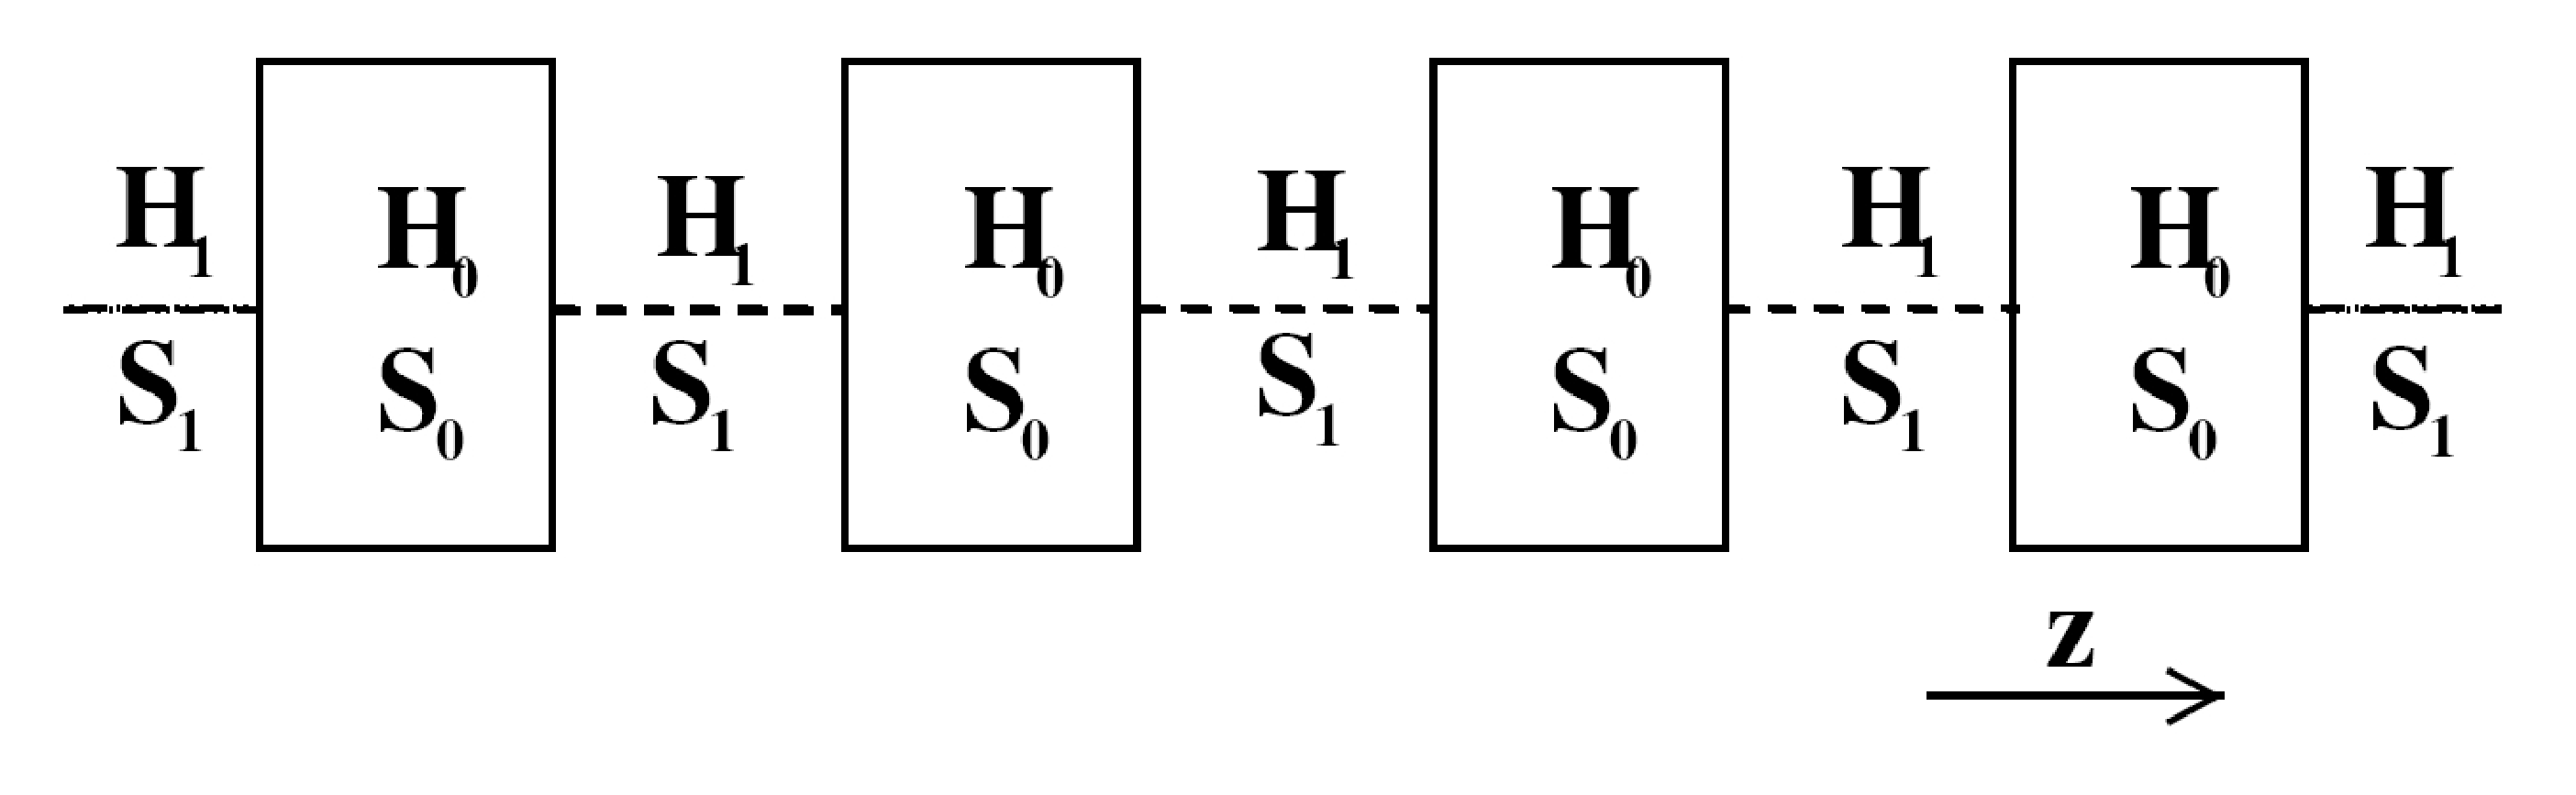
\includegraphics[width=9.0cm,clip=true]{fig/Fig2}
\caption{Periodic structure of the leads. $H_0$ and $S_0$ are the Hamiltonian and overlap matrix describing
the interaction within one unit cell and $H_1$ and $S_1$ are the coupling and overlap matrix describing the
interaction between adjacent unit cells. The arrow shows the direction of transport ($z$ direction).
}
\label{fig:leads}
\end{figure}
%*****************************************************************


Here SMEAGOL evaluates the Hamiltonian $H$, the overlap $S$ and the density matrices $\rho$ of the current/voltage probes (the leads). The self-energies for the semi-infinite electrodes can be obtained from the knowledge of the Hamiltonian and the overlap matrices of an infinite system, and therefore only a DFT calculation for a bulk system is needed. $H$ and $S$ should be written in the tridiagonal form described by Sanvito et al. [1, 14]. Figure (2) shows the typical setup for the electrodes.  The same procedure is used for calculating the matrix elements of the Hamiltonian and overlap matrix in the case of k-points calculation (along the direction orthogonal to transport).

\subsection{Input files}
There are no additional input files than those used by SIESTA for an ordinary DFT calculation (input file, pseudopotentials ...). For these we refer to the SIESTA user guide. 

\subsection{Input flags}
The following input flags must be supplied to the \filestyle{input.fdf} file in order to perform the bulk calculation.\\
\vspace{0.3cm}

\inputflag{BulkTransport}{Boolean}{When this flag is set to true the leads Hamiltonian and overlap matrix will be written to the file \filestyle{SystemLabel.HST}. Moreover the files \filestyle{bulklft.DAT} or \filestyle{bulkrgt.DAT} (or both) will be created. These contain information about the system (Fermi energy, System label, unit cell, non-zero elements of the Hamiltonian and information about the super cell).}{F}

\inputflag{BulkLeads}{String}{Should always be set to "LR".}{LR}

\subsection{Output files}

\vspace{0.5cm}
\filedescription{bulklft.DAT}
{File containing information about the left-hand side lead (number of states, Fermi energy, number of $k$-points, etc)}

\filedescription{bulkrgt.DAT}
{File containing information about the right-hand side lead (number of states, Fermi energy, number of $k$-points, etc)}

\filedescription{Systemlabel.HST}
{File containing the Hamiltonian and overlap matrices of the leads. The string Systemlabel is read from either \filestyle{bulklft.DAT} or \filestyle{bulkrgt.DAT}. If the two leads are the same one can use the same \filestyle{Systemlabel.HST} file to read the information for both the left and right leads. If the two systems are different, then two files with different names must be provided from two different leads calculations. The usage for different electrodes is outlined in Sec. \ref{sec:diffele}.}

\filedescription{Systemlabel.DM}
{File containing the density matrix of the leads. It is needed for calculating the $I$-$V$ . The string Systemlabel is read from either \filestyle{bulklft.DAT} or \filestyle{bulkrgt.DAT}. If the two leads are made from the same materials and have the same geometrical arrangement one can use the same \filestyle{Systemlabel.DM} file to read the information about both the left- and righthand side lead. If the two leads are different, then two files with different names must be provided from two independent leads calculations. The usage for different electrodes is outlined in Sec. \ref{sec:diffele}. The \filestyle{Systemlabel.DM} file is used to set the boundary condition at the interface between the scattering region and the electrodes.}

\section{\textit{I-V} calculation}

Once the initial calculation for the leads has been performed we can proceed with computing the non-equilibrium transport properties of our system.
%*****************************************************************
\begin{figure}
\center
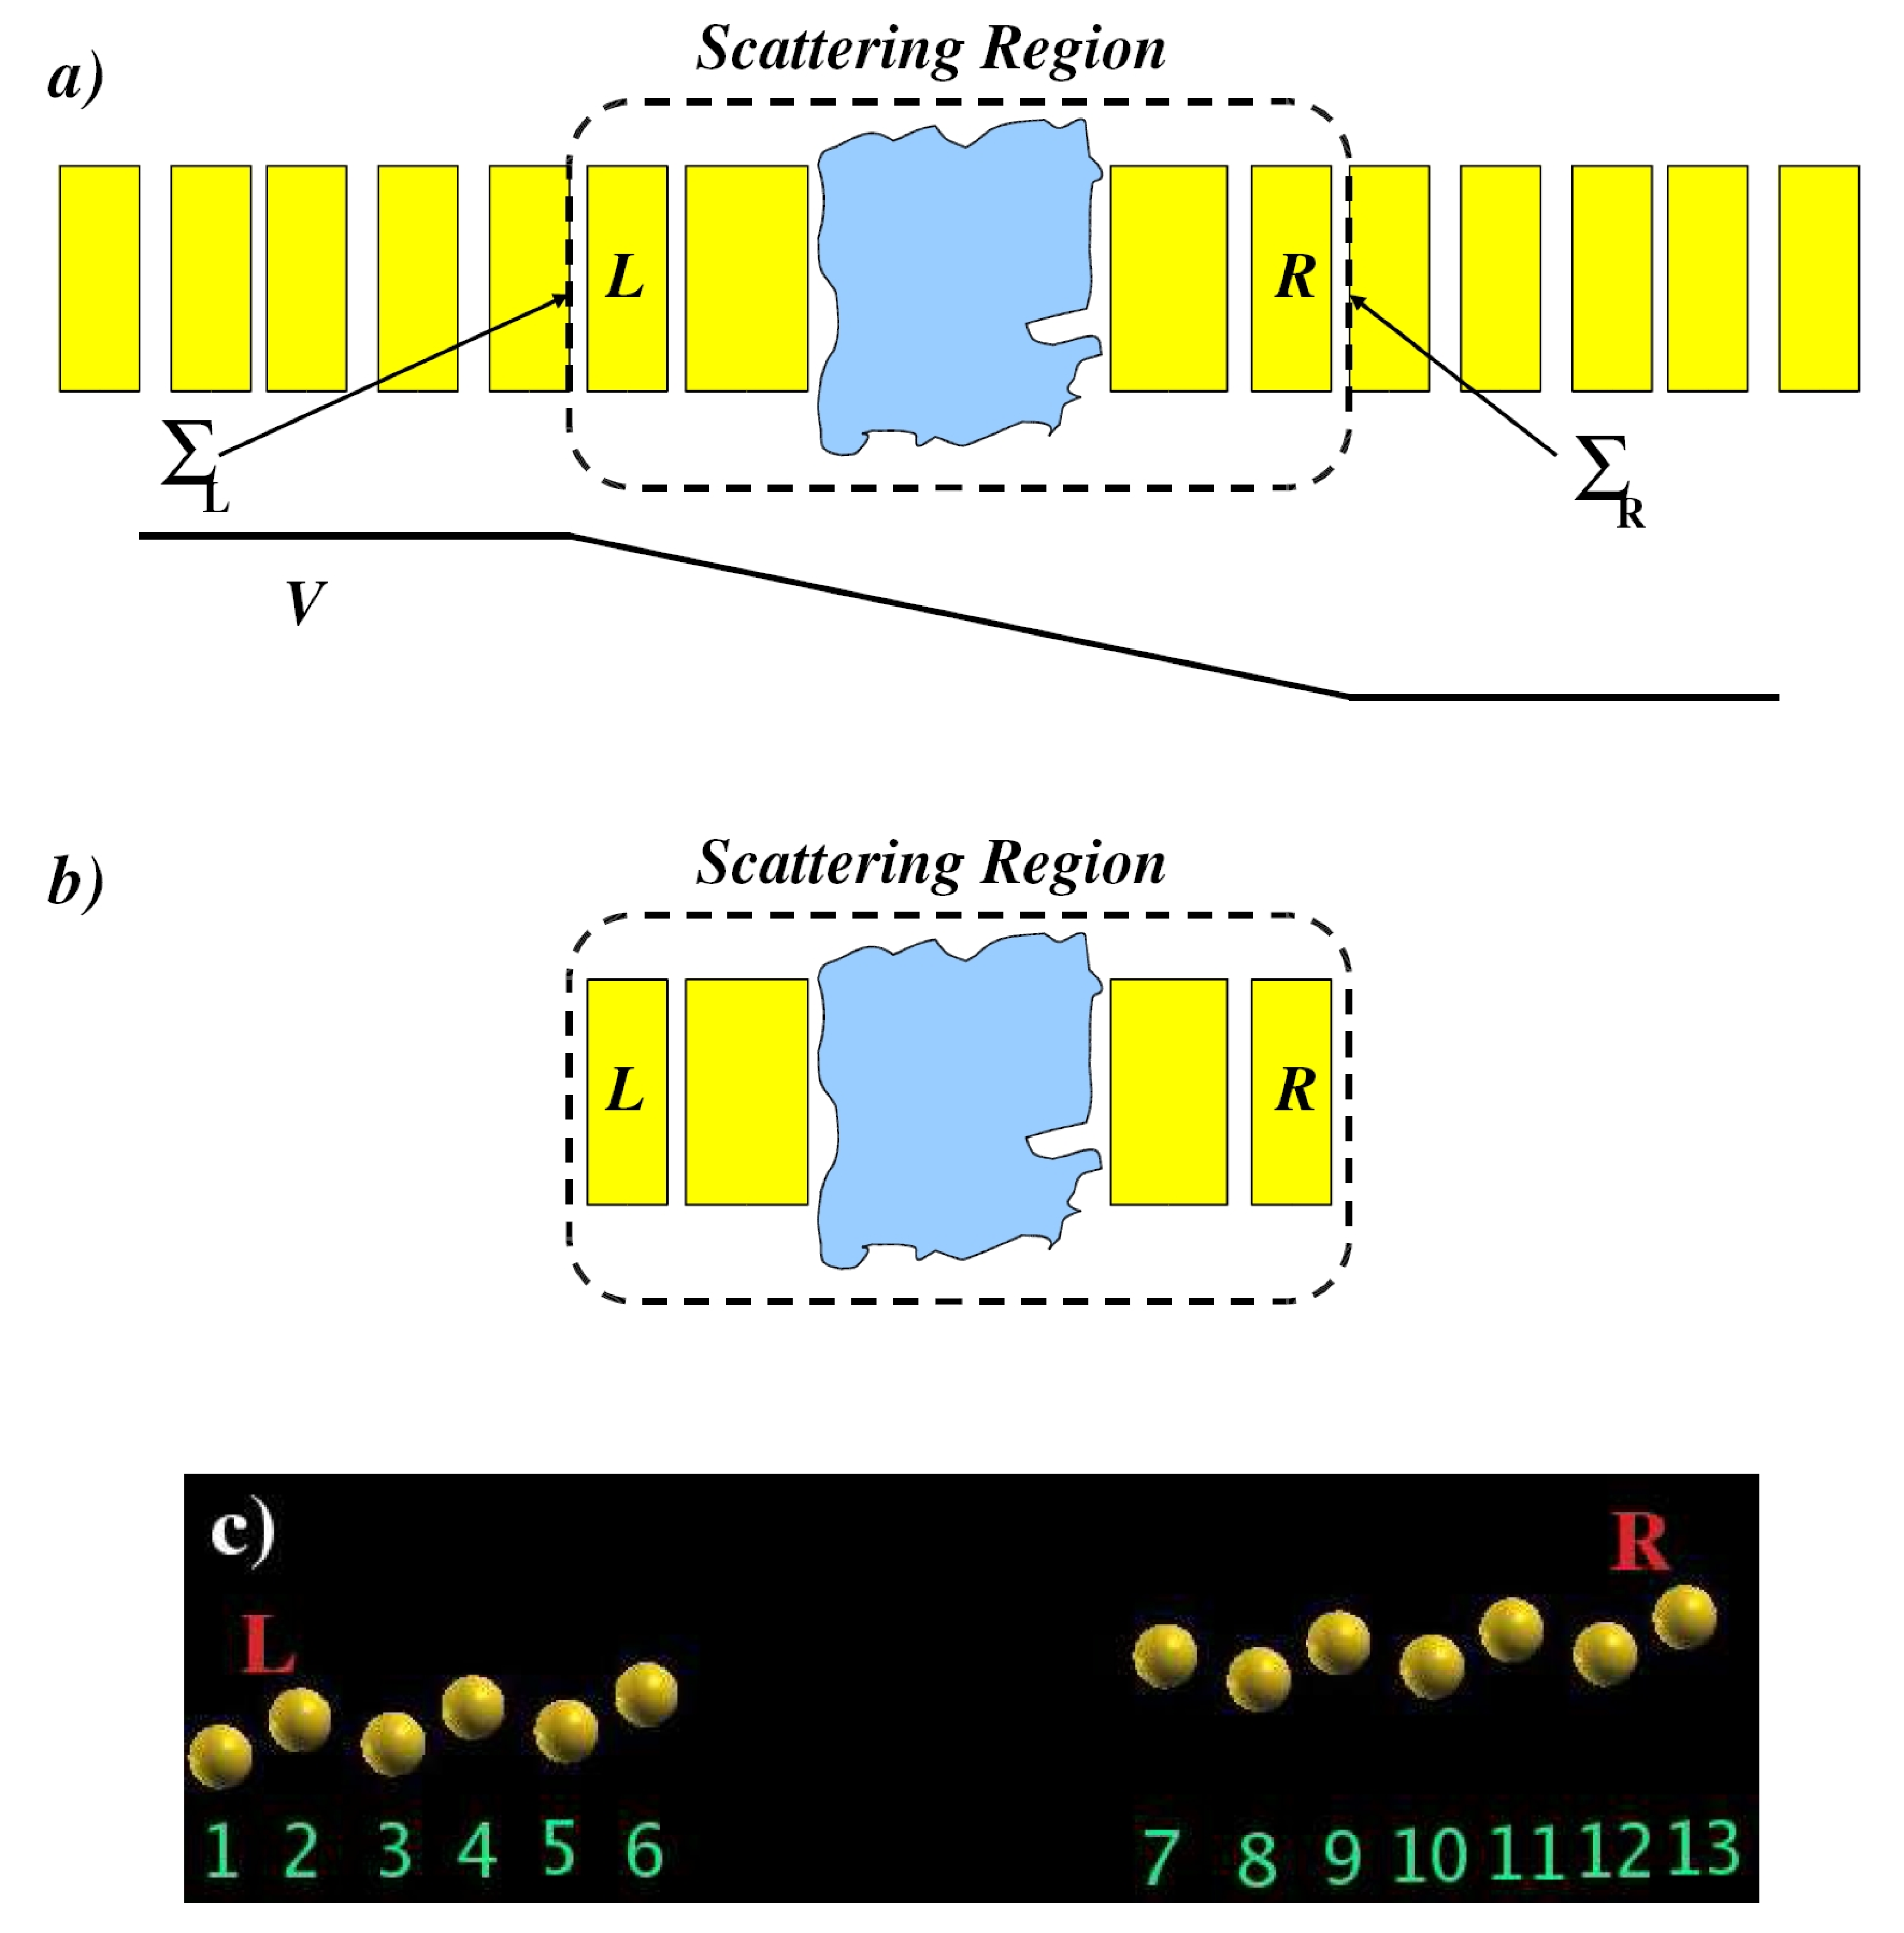
\includegraphics[width=10.5cm,clip=true]{fig/Fig3}
\caption{a) Sketch of a typical system simulated using SMEAGOL: two semi-infinite electrodes connected
to a central scattering region. b) The typical unit cell for a SMEAGOL calculation. The reader
must note that we include at least one layer of the leads both to the left- and to the right-hand side of
the scattering region. The order of the atoms in the input file is only important in these two layers. The
first atoms of the list (see AtomicCoordinatesAndAtomicSpecies in the SIESTA user guide) must be
those contained in the left-hand side lead unit cell, and they must be input with the same order than
in the bulk leads calculation. In an analogous way, the last atoms of the list must conform with the
input file for the right-hand side lead. c) An example of a system setup for two semi-infinite zig-zag wires
separated by a vacuum region. The numbers for each atom have been indicated as well as the two atoms
on either side corresponding to the the unit cells for the left- and right-hand side lead.}
\label{fig:system}
\end{figure}
%*****************************************************************


\subsection{Input files}
Several files generated during the construction of the leads must be used. These are: \filestyle{bulklft.DAT}, \filestyle{bulkrgt.DAT}, \filestyle{Systemlabel.HST} and \filestyle{Systemlabel.DM}.

\subsection{Input flags}
The following input flags must be supplied to the file \filestyle{input.fdf} in order to perform the transport ($I$-$V$) calculation. If any of these values is not supplied, the default value will be assumed.  Special care should be taken for the variables that control the real and contour integrals, when calculating the non-equilibrium density matrix.

\vspace{0.5cm}
\inputflag{EMTransport}{Boolean}
{When {\bf EMTransport} is set to T, SMEAGOL will perform a NEGF calculation (transport).  Otherwise, the code will perform a standard SIESTA equilibrium ground state calculation for either a periodic system or a molecule.}
{F}

%*****************************************************************
\begin{figure}[h]
\center
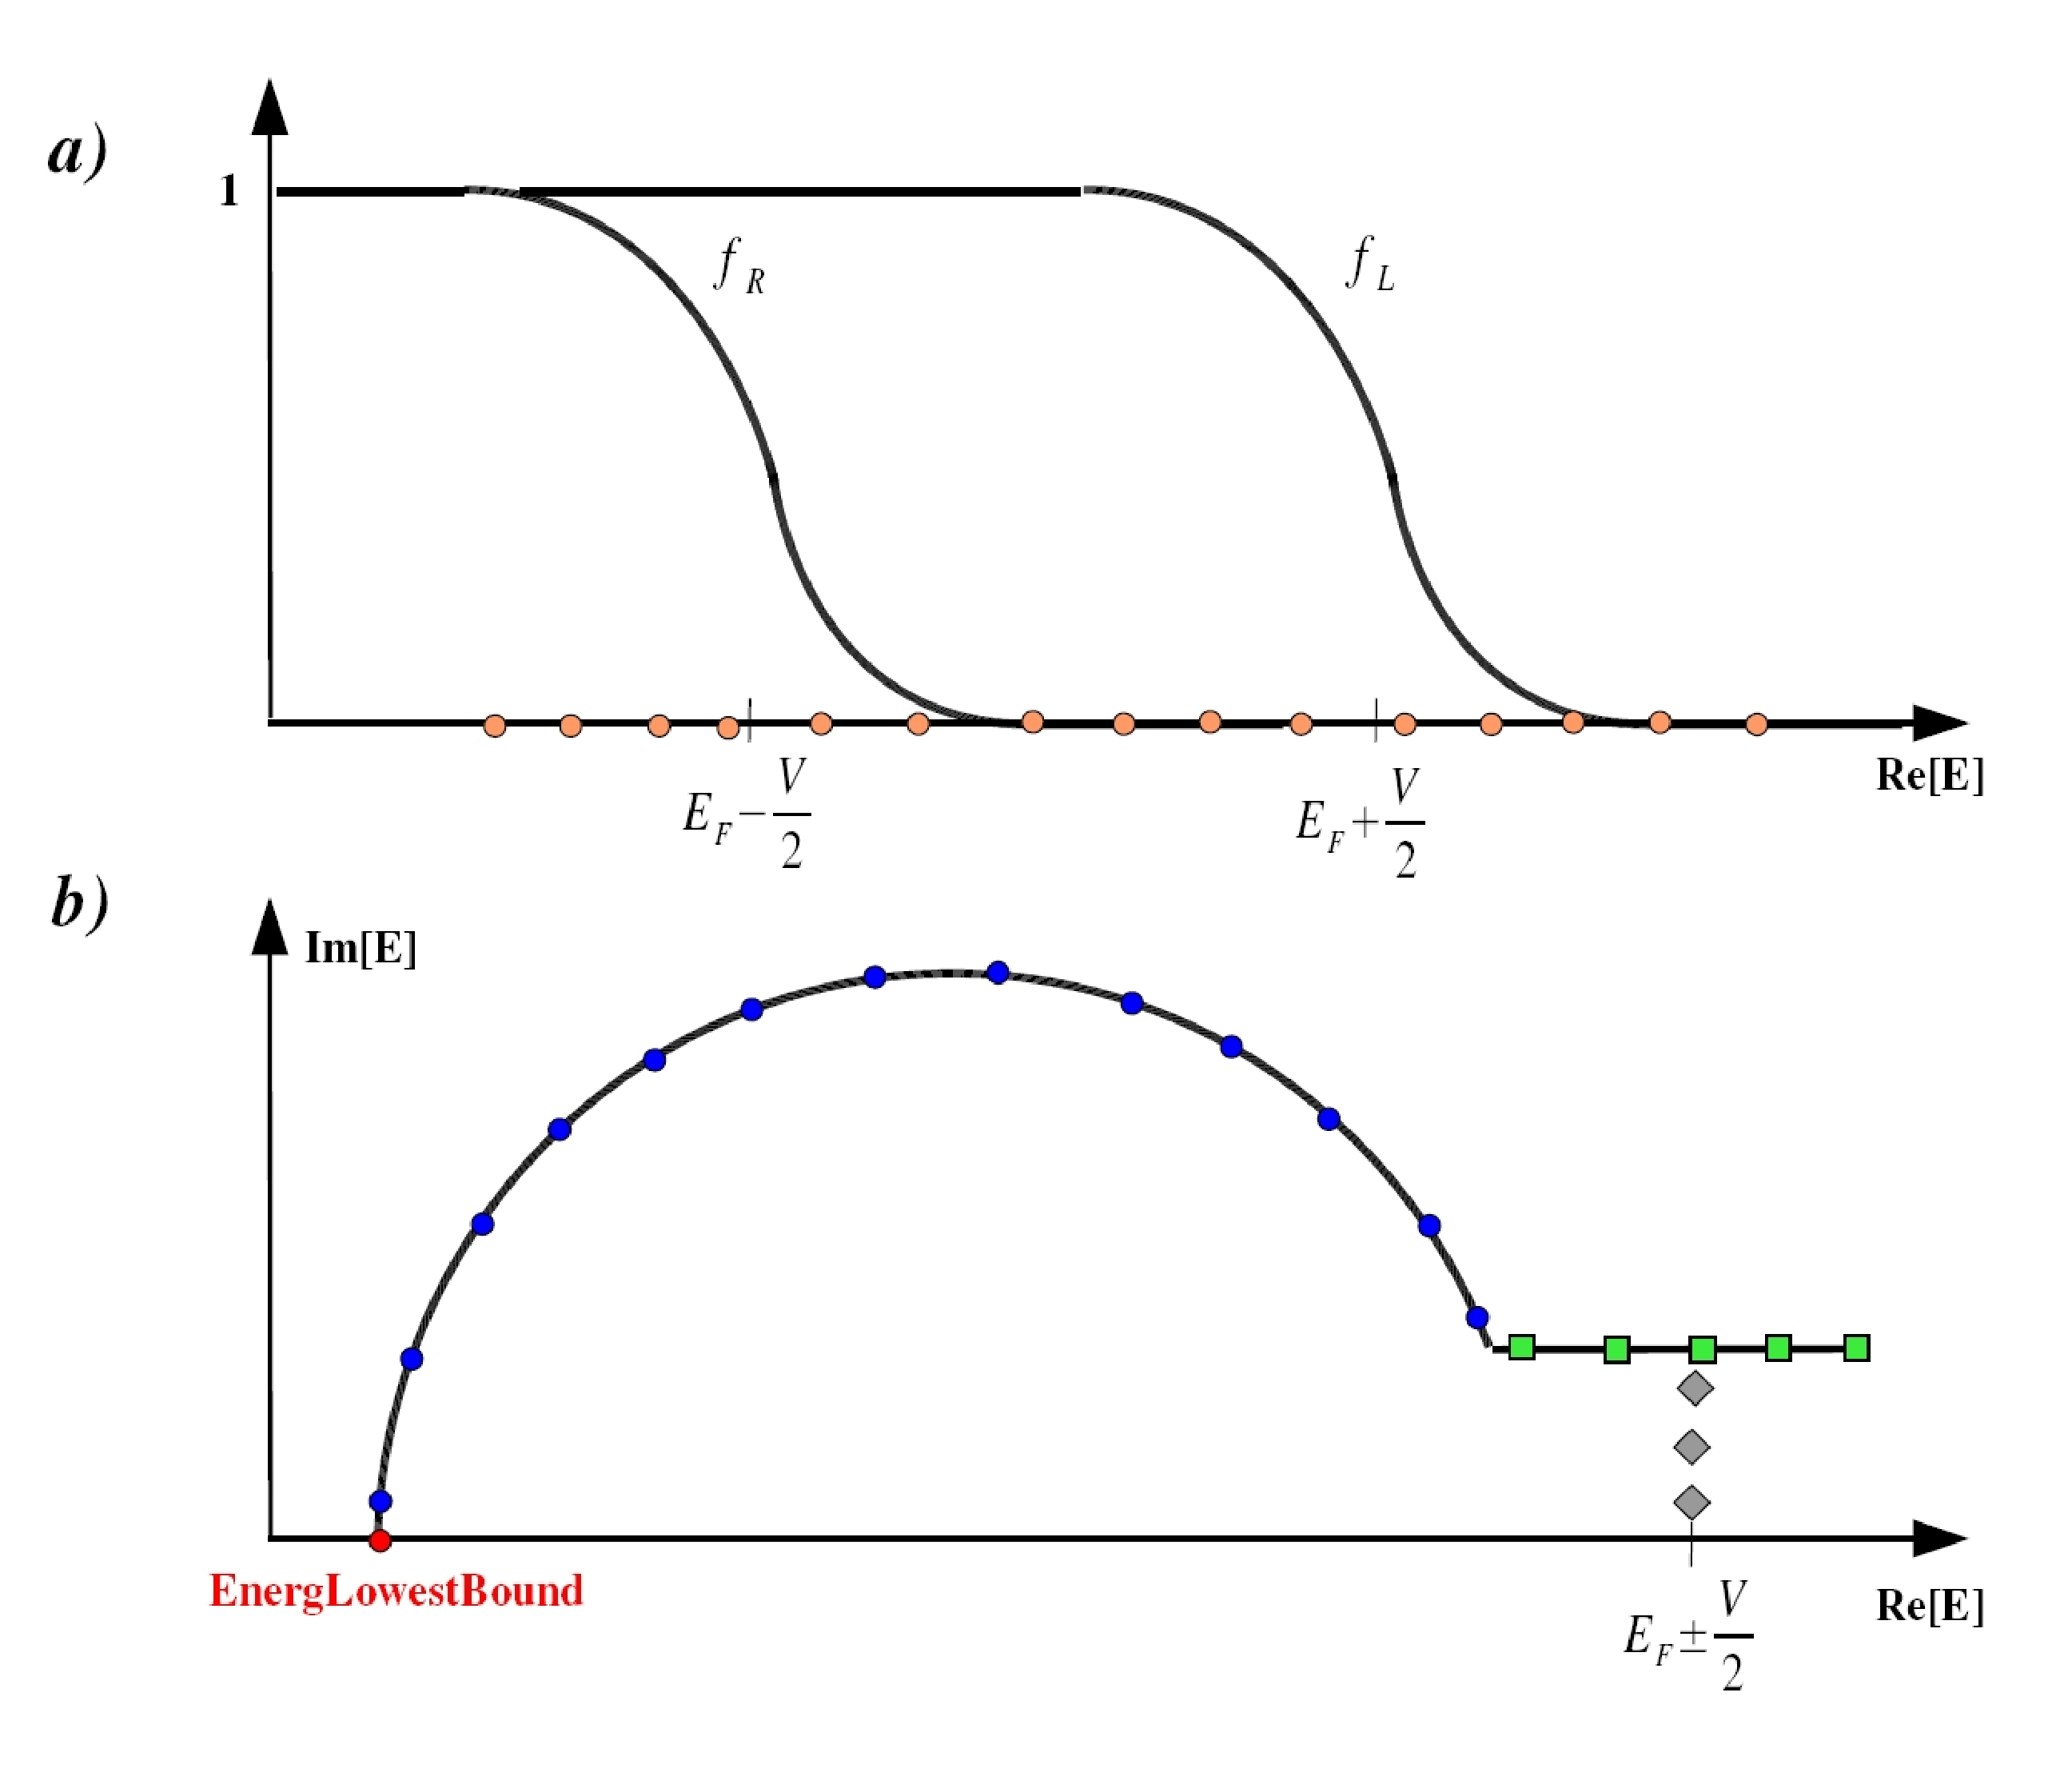
\includegraphics[width=10.5cm,clip=true]{fig/Fig4}
\caption{ Sketches for the Green Function integration leading to the non-equilibrium charge density
[1, 2]. a) The non-equilibrium part must be performed along the real energy axis, but is bound by the
left- and right-hand side Fermi distributions functions, $f_L$ and $f_R$. b) The equilibrium component is
performed over a semicircular path in the complex energy plane. Here we show the starting position
EnergLowestBound, the energy mesh along the two segments of the curve and the poles of the Fermi
distribution.  }
\label{fig:integral}
\end{figure}
%*****************************************************************
\inputflag{NEnergReal}{Integer}
{Number or energy points along the real axis for the integration of the non-equilibrium part of the Green's function. The number of points is extremely sensitive to the type of calculation performed. The points are distributed between $-(V/2 + 30.0 k_B T)$ and $+(V/2 + 30.0 k_B T)$. The number of points determines how fine the mesh is. Since the Green's function on the real axis can be ill-behaving (large number of singularities), a very fine mesh might be necessary. For equilibrium calculations, NEnergReal can be set to zero. In Fig. (4a) the real axis energy points are sketched as orange circles and NEnergReal= 15.}{0}

\inputflag{NEnergImCircle}{Integer}
{Number of energy points along the semi-circle in the complex plane (equilibrium part of the Green's function integral). The circle starts at the energy EnergLowesBound and finishes at the complex point energy point ($E_F - 30.0 k_BT$, $2~\mathrm{NPoles}~k_BT$). The values for the energy points are calculated using a Gauss-Legendre algorithm along a semicircle. Fig.  (4b) shows a sketch of the points along the contour in the complex energy plane. In this example, the points along the circle are represented by blue circles and NEnergImCircle= 13.}
{16}

\inputflag{NEnergImLine}{Integer}
{Number of energy points along the line in the complex plane where the integral of the equilibrium contribution to the density matrix is performed. This straight line starts at the point ($E_F - 30.0 k_BT$, $2~\mathrm{NPoles}~k_BT$) and finishes at point ($E_F + 30.0 k_BT$, $2~\mathrm{NPoles}~k_BT$) (green squares in Fig. (4b), NEnergImLine= 5). The position of the energy points is determined by a Gauss-Legendre algorithm.}
{16}

\inputflag{NPoles}{Integer}
{Number of poles in the Fermi distribution used to compute the contribution to the equilibrium charge density. The Fermi distribution is given by:
f (x) = 1 e −μ kBT + 1 (1)
\begin{equation}
f(x)=\frac{1}{e^{\frac{e-\mu}{k_BT}}+1}
\end{equation}
The poles of $f(e)$ all lay on the complex plane with $i_n = \mu + (2 n + 1) i \pi$ being the $n$-th pole. The number of poles specifies how far from the real axis the contour integral will be performed. The furthest away from the real axis the more well-behaving the Green's function is.  In Fig. (4b) the position of the poles are represented by grey diamonds (NPoles= 3).}
{16}

\inputflag{VInitial}{Physical}
{Value of the initial bias for the $I$-$V$ calculation.}
{0.0 eV}

\inputflag{VFinal}{Physical}
{Value of the final bias for the $I$-$V$ calculation.}
{0.0 eV}

\inputflag{NIVPoints}{Integer}
{Number of bias steps considered between the two limits Vinitial and Vfinal. The current will be calculated only for these biases.}
{0}

\inputflag{Delta}{Double precision}
{Small imaginary part $\delta$ that accounts for the broadening of the localized energy levels of Green's Function, $G=\left[(E+i\delta)S-H-\Sigma_L-\Sigma_R\right]^{-1}$.}{1.0e-10}

\inputflag{EnergLowestBound}{Physical}
{Energy that specifies the beginning of the contour integral in the complex plane for the equilibrium contribution to the charge density. EnergLowestBound must be below both the lowest band of the leads and the lowest energy level of the scattering region. Red dot in Fig. (4b).}
{-7.0 Ry}

\inputflag{AtomLeftVCte}{Integer}
{Number of the atom used to determine the onset of the bias ramp on the left-hand side.  The number of the atom is taken from the order in which the atoms are specified in the SIESTA block AtomicCoordinatesAndAtomicSpecies (refer to the SIESTA manual for a description of this block).}
{1}

\inputflag{AtomRightVCte}{Integer}
{Number of the atom that is used to determine the onset of the bias ramp on the right-hand side. The number of the atom is taken from the order in which the atoms are specified in the SIESTA block AtomicCoordinatesAndAtomicSpecies (refer to the SIESTA manual for a description of this block).  For $z < z_\mathrm{AtomLeftVCte}$ and $z > z_\mathrm{AtomRightVCte}$, the potential added to the Hartree potential is a constant equal to +$V/2$ and -$V/2$, respectively. For $z_\mathrm{AtomLeftVCte} < z < z_\mathrm{AtomRightVCte}$ a bias ramp $V (z - z_0)$ is introduced, where $z_0$ is the midpoint between $z_\mathrm{AtomLeftVCte}$ and $z_\mathrm{AtomRightVCte}$.}
{Last Atom}

\inputflag{TrCoefficients}{Boolean}
{If set to true the transmission coefficients as a function of energy $T(E,V)$ will be calculated and printed to the file \filestyle{Systemlabel.TRC} (see section 4.3 below) for every bias point.  Although the current is defined as
e h Z 1 −1 T (, V) (fL − fR) d (2)
\begin{equation}
\frac{e}{h}\int_{-\infty}^{\infty}T(E,V)\left(f_L-f_R\right)dE
\end{equation}
we can calculate the Transmission coefficients for a wider range of energy values and a different number of energy points by using the variables InitTransmRange, FinalTransmRange and NTransmPoints which are defined below.}
{F}

\inputflag{InitTransmRange}{Physical}
{Initial energy for the calculation of the transmission coefficients.}
{-5.0 eV}

\inputflag{FinalTransmRange}{Physical}
{Final energy for the calculation of the transmission coefficients.}
{5.0 eV}

{\inputflag{NTransmPoints}{Integer}
{Number of energy points uniformly distributed between InitTransmRange and FinalTransmRange for which the transmission coefficients are calculated. If TrCoefficients is set to false, this flag is ignored.}
{100}

\inputflag{SaveBiasSteps}{data block}
{Block containing information for printing the Hartree potential (\filestyle{Systemlabel.VH}), the charge density (\filestyle{Systemlabel.RHO}), the difference between the self-consistent and the atomic charge densities (\filestyle{Systemlabel.DRHO}) and the total DFT potential 9 (\filestyle{Systemlabel.VT}) at a specified bias step. The arguments in the block are integers indicating the bias steps at which to print these files. They range from from 0 up to NIVpoints.  The appropriate SIESTA flag for printing any of these files must also be set to true.

\begin{flushleft}
Example:\linebreak
{\ttfamily
\%block SaveBiasSteps\linebreak
0 2 3\linebreak
\%endblock SaveBiasSteps}
\end{flushleft}
SMEAGOL will print the requested file (for instance \filestyle{Systemlabel.VT} if the SIESTA flag SaveElectrostaticPotential is set to true) at the bias steps 0, 2 and 3.}
{No Default}

\subsubsection{Matching of the Hartree Potential}

One important information needed from the leads calculation is the average value of the Hartree Potential. SMEAGOL uses a Fast Fourier Transform (FFT) algorithm to solve the Poison equation in reciprocal space (refer to the SIESTA manual for more details). The ~k = 0 term is ignored resulting in a Hartree Potential that is defined up to a constant. This might lead to a mismatch between the Hartree potential of the leads and that at the edges of the scattering region. This mismatch is better illustrated in Fig. 5 where we have plotted the average Hartree potential on the plane orthogonal to transport for the electrodes and two semi-infinite wires separated by 12 \AA~(our scattering region; see Fig. (3c)) using the post-processing tool Pot.exe (included in the Utils directory).  In order to compensate for the arbitrary zero of the potential we shift the Hartree Potential of the scattering region by a constant (see variables HartreeLeadsLeft, HartreeLeadsRight and HartreeLeadsBottom described below). In this way we force the match of the potential at the scattering region/leads interface.
%*****************************************************************
\begin{figure}
\center
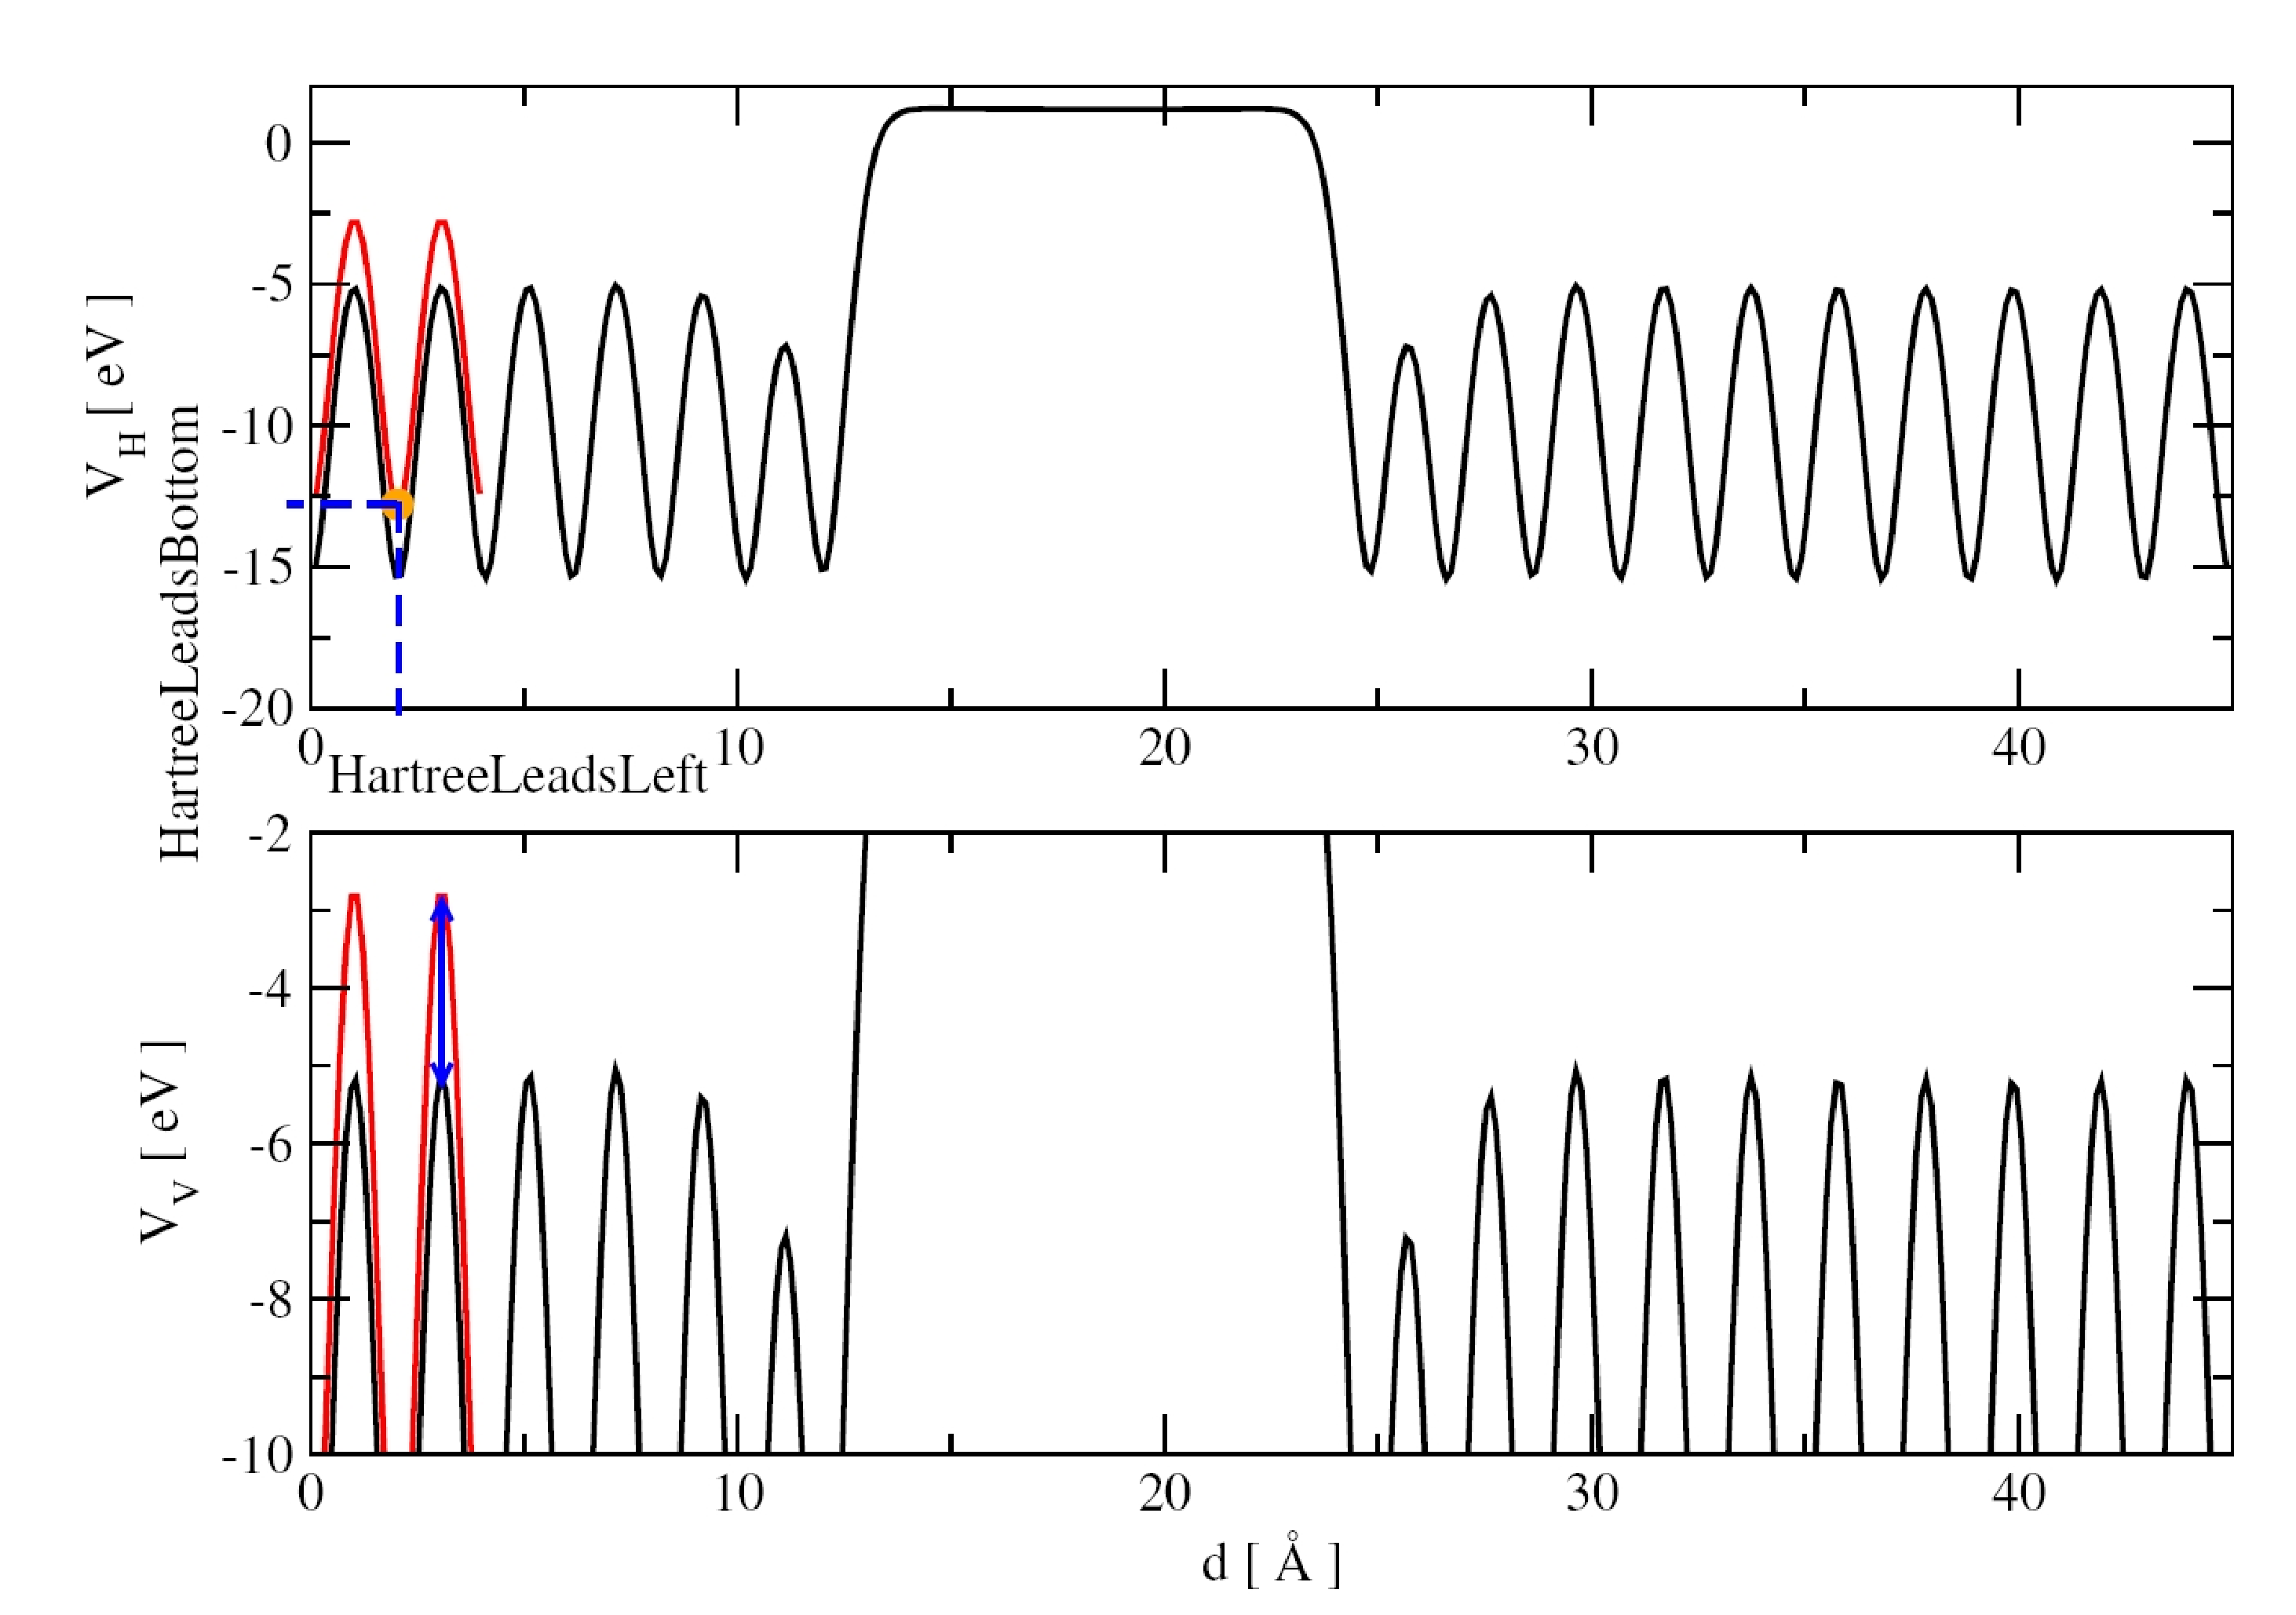
\includegraphics[width=9.5cm,clip=true]{fig/Fig5}
\caption{Shift of the Hartree potential between two SIESTA calculations: bulk gold (the leads)
with two atoms in the unit cell (red line) and the parallel plate capacitor (scattering region)
depicted in Fig. (3c). Note that the Hartree potential of the scattering region has converged to
the bulk value after the first atomic layer except for a constant.}
\label{fig:potential}
\end{figure}
%*****************************************************************


\inputflag{HartreeLeadsLeft}{Physical}
{Position in space in the left-hand side lead where the Hartree potential of the scattering region should match that of the bulk.}
{0.0 Ang}

\inputflag{HartreeLeadsRight}{Physical}
{Position in space of the right-hand side lead where the Hartree potential in the scattering region should match that of the bulk.}
{0.0 Ang}

\inputflag{HartreeLeadsBottom}{Physical}
{Average value of the Hartree potential in the leads over a plane perpendicular to the transport direction. This parameter should be evaluated from the bulk leads calculation. The fast Fourier Transform algorithm used in SMEAGOL to solve the Poisson’s equation disposes the k = 0 term. This defines the Hartree potential up to an arbitrary constant. By defining HartreeLeadsBottom we shift the Hartree potential in the scattering region in order to match that of the leads.}
{0.0 eV (no shift)}

\subsubsection{Flags specific of $k$-point calculations}
These flags are used only when periodic boundary conditions in the direction orthogonal to the transport are considered.

\vspace{0.5cm}
\inputflag{SaveMemTranspK}{Boolean}
{By default, SMEAGOL calculates the self-energies during the first iteration and stores them in memory. There are two self-energies (one for the left- and one for right-hand side contact) for each energy point and each $k$-point. If the number of $k$-points and the size of the unit cell of the leads are large, large memory might be needed. In that case, SaveMemTranspK should be set to T, and the self-energies will be re-calculated after each iteration without the need for storing them in memory. Use with caution; this specification might increase considerably the time of the calculation.}
{F}

\inputflag{TransmissionOverk}{Boolean}
{Allow to print the transmission coefficient as a function of both the k-vector in the transverse Brillouin zone and the energy. Note that the flag TrCoefficients provide only the 11 integral of the transmission coefficients over the $k$-points. TrCoefficients must be set to true. The file \filestyle{Systemlabel.TRC.k.up} (down) contains the results (see section 4.3 below).}
{F}

\subsection{Output files}

\filedescription{SystemLabel.CUR}
{Four column vector containing the $I$-$V$ characteristics. The first column corresponds to Transmission coefficients as a function of energy for different biases. The first column corresponds to the energy, the second to the total transmission for both the spin direction and the following nspin columns are the spin-decomposed transmission coefficients.}

\filedescription{SystemLabel.TRC.k.up (down)}
{If TransmissionOverk is set to T, \filestyle{Systemlabel.TRC.k.up} contains the transmission coefficients for each $k$-point and energy for either up or down spins. The first two columns contain the perpendicular components of each $k$-point, the third column contains the weight for this $k$-point, the fourth column contains the spin dependent transmission coefficient and the fifth column contains the energy in eV with respect to the Fermi energy. The 6th (7th) column contains the number of channels of the left (right) electrode for this $k$-point and energy.}

\filedescription{SystemLabel.CHR}
{File containing the total charge inside the scattering region after each iteration. The first column contains the iteration number, the second column contains the charge in units of e (the electron charge), the third column contains the bias in Rydberg and the fourth column contains the temperature also in Rydberg.}

\filedescription{IV.SystemLabel.VH}
{If SaveElectrostaticPotential is set to true (see SIESTA user guide) and the block SaveBiasSteps is present, the file \filestyle{IV.Systemlabel.VH} containing the Hartree potential for the biases specified in SaveBiasSteps will be generated.}

\filedescription{IV.SystemLabel.VT}
{If WriteVT is set to true (see SIESTA user guide) and the block SaveBiasSteps is present, the file \filestyle{IV.SystemLabel.VT} containing the total DFT potential for the biases specified in SaveBiasSteps will be generated.}
\filedescription{IV.SystemLabel.RHO}
{If WriteRHO is set to true (see SIESTA user guide) and the block SaveBiasSteps is present, the file \filestyle{IV.Systemlabel.RHO} containing the self-consistent charge density for the biases specified in SaveBiasSteps will be generated.}
\filedescription{IV.SystemLabel.DRHO}
{If WriteDRHO is set to true (see SIESTA user guide) and the block SaveBiasSteps is present, the file \filestyle{IV.Systemlabel.DRHO} containing the difference between the selfconsistent and the atomic charge densities for the biases specified in SaveBiasSteps will be generated.}
\filedescription{IV.SystemLabel.DMT}
{If SaveDMT is set to true and the block SaveBiasSteps is present, the file \filestyle{IV.Systemlabel.DM} containing the converged density matrix at each bias specified in SaveBiasSteps will be written.}

\section{How to run smeagol}

Assuming that the user has already compiled SMEAGOL successfully and saved it as an executable (say smeagol.1.2), then we are ready to start a calculation. Initially the user must setup the input file for the left- and right-hand side leads. The input file must include the appropriate SIESTA and SMEAGOL flags as discussed in section (3.2) and in the SIESTA Manual. Let us assume, as a simple example, that the two leads are equivalent and the leads file is called leads.fdf. In the same directory where this file is, there must also be the pseudopotential files - either in .psf or .vps format. Then the user should type:\\
{\ttfamily \$ smeagol.1.2 < leads.fdf > leads.out}\\
The calculation will yield the files \filestyle{bulklft.DAT}, \filestyle{bulkrgt.DAT}, \filestyle{Systemlabel.HST} and\\ \filestyle{Systemlabel.DM} These should be moved to the directory containing the input file for the scattering region - say scattering.fdf. This directory must also contain pseudopotential files for all the atomic species involved in the calculation. It is important to note that the user must be consistent with regards to pseudopotentials, they should be identical to the ones used for the leads calculation.  Before starting the $I$-$V$ calculation we must obtain HartreeLeadsBottom. For that we use the post-processing tool Pot.exe contained in the Utils directory of the SMEAGOL distribution.  The file Potential.dat should be edited in order to process the file \filestyle{Systemlabel.VH} (for the leads). The resulting output \filestyle{Systemlabel.VH} can be viewed using a plotting tool such as gnuplot or xmgrace.  We are interested in the first two columns of this data file. They contain the planar average of the Hartree potential as a function of the $z$ direction. A value for the Hartree Potential (HartreeLeadsBottom) should be chosen (usually the edges of the unit cell) and the position in the unit cell should be recorded and matched with the equivalent position in the scattering region (HartreeLeadsLeft and HartreeLeadsRight). Once this is done, we are ready to calculate the $I$-$V$ characteristics:\\
{\ttfamily \$ smeagol.1.2 < scattering.fdf > scattering.out}\\
The resulting files can be processed using a variety of plotting programs such as gnuplot and xmgrace for 2D-plots and OpenDX for 3D-plots and isosurfaces.




\section{Changes compared to smeagol-1.0b}

This code (smeagol-1.2) is a development version. If you encouter
problems please write to runggeri@tcd.ie.

Here are a few notes on the main changes from the distribution version smeagol-1.0b, which is described in the file \filestyle{Smeagol-1.0.pdf}. Some of the options listed in the \filestyle{Smeagol-1.0.pdf} have been removed, and some have changed the default values. 


1) SMEAGOL now uses both the density matrix (.DM) and the Hamiltonian (.HM)
file to restart calculations. It is important that both the .DM and .HM file
are from the same step in the calculation for good convergence. Convergence now takes a similar amount of scf iterations as for {\bf EMTransport} F. Sometimes if there are convergence problems killing
and restarting the calculation helps (because then it starts from a matching
pair of .DM and .HM files).

2) By default this code applies the potential-ramp from $z$=0 to $z$="length of unit cell" (You can set the option FullRamp to False to prevent this, but
there should never be a reason to do this). This is the correct way to do
apply the ramp, and one needs to make sure that the left lead starts at approximately $z$=0.

A non-self-consistent rigid shift potential drop can be applied by setting
FullRamp to false, and choosing appropriate values for AtomLeftVcte and AtomRightVcte.
Moreover, the value for MaxSCFIterations has to be set to 1, so that the
self-consistent loop is not entered. In this case the potential drop is
applied between the positions of AtomLeftVcte and AtomRightVcte. As already
mentioned, FullRamp should not be set to False in a self-consistent
calculation, since it would leads to unphysical results.

3) A new method is used to construct the selfenergies, it is described in Ref.  I. Rungger and S. Sanvito, Phys Rev B 78, 035407 (2008).  This is one of the major improvements in the code compared to the standard distribution version of SMEAGOL, therefore please cite the paper if you use this code. You can still use the old method by setting Sigma.Method 0.

4) In the calculation of the transmission coefficient in the .TRC file, the
Fermi energy is set to 0, and the unit of the energy axis is in eV. If
k-points are used, the transmission coefficient and number of channels is
rescaled by the number of k-points. If the transmission coefficient is
calculated at different bias steps, then for each bias step it is written in a
separate file, where the number of the bias step is added as prefix. One (two
in case of a spin polarized calculation) new column is appended in the .TRC
file, and corresponds to the number of channels of the right lead. Moreover,
in the .CUR file, where the $I$-$V$ is written, the units of the voltage is Volts.

Further improvements include the possibility to calculate the PDOS at finite bias, to perform a decomposition of the transmission into transmission channels and plot the corresponding transmission wave functions. Moreover the code works in parallel for systems with non-collinear spins and systems including spin-orbit interaction. It is possible to evaluate the spin transfer torque. Note that many new features have been added to the development version as compared to the standard distribution version, which are not yet documented in this user guide.
%\subsection{Inclusion of bound states}
%
%In Fe/MgO/Fe and similar junctions there are bound states at each of the two
%interfaces between the metal and the MgO (there are bound states on the left
%and on the right interface). If BS.Add is set to True, then at finite bias the
%code simply occupies all the bound states on the left up to the left Fermi
%energy, and the ones on the right up to the right Fermi energy. To do this the
%code needs to know what is on the left, and what on the right. The way it is
%implemented now, you first have to sort the atoms in the input file from left
%to right (you probably already did it). Then by default the code just takes
%the middle orbital of the Hamiltonian, and all the elements with a smaller
%index are considered to be on the left, and oll the other ones are considered
%to be on the right. Moreover, the bound states are broadened using the
%specified value of Delta, the number of energy points on the real axis
%therefore has to be large enough, in order to resolve peaks with a width of
%about Delta. Usually I would use Delta 1.0e-4 Ry, so that you need at least
%about 1 energy point every meV. For a bias of 1 Volt I therfore suggest to use
%about 3200 energy points. This method works very well generally for interface
%states/surface states.
%
%The relevant fdf options are:
%\vspace{0.5cm}
%
%\inputflag{BS.Add}{Boolean}
%{if set to true the bound states correction is added. The default is
%.false., you therefore have to set it to true explicitely in the calculation to include the bound states.}{False}
%
%\inputflag{BS.MiddleOrbital}{Integer}
%{this option takes an integer number (default 0). If the junction is not symmetric, then you have to specify by hand which orbital is in the middle of the junction. To find this out you have to open the output file of a previous calculation (for example the 0-bias one) and look for the lines starting with "label:". There is a list of atomic orbitals and their index. From there you can select which index corresponds to the middle of the junction. If the junction is symmetric you don't need this option, or you set the value to 0, then the middle orbital is used to separate left from right.}{Middle orbital}
%
%That is it. This code works for simple tunneling junctions. For double
%junctions or more fancy stuff one would have to extend it. The example input
%files I sent you last time are set up to correctly include the bound states
%for the different bias voltages.
%
%************************************
%
%List of related new fdf-options:
%\vspace{0.5cm}
%
%\inputflag{BS.Add}{Boolean}
%{If set to T, the code adds the bound states correction.}
%{F}
%
%\inputflag{BS.MiddleOrbital}{Integer}
%{Index of the orbital that divides the junction into left and right part. If set to 0, the middle orbital is used (this is the standard for symmetric junctions).}
%{0}
%
%List of undocumented new fdf-options:
%\vspace{0.5cm}
%
%\inputflag{EM.OneKP}{Integer}{}{0}
%
%\inputflag{Sigma.Tolab}{Double}{}{1d-6}
%
%\inputflag{UseLeadsGF}{Boolean}{}{F}
%
%\inputflag{BS.Method}{Integer}{}{1}
%
%\inputflag{BS.Tolerance}{Double}{}{1D-5}
%
%\inputflag{BS.Minimum}{Double}{}{0D0}
%
%\inputflag{SetEnergyRange}{Boolean}{}{F}
%
%\inputflag{SetEmin}{Double}{}{-1D0}
%
%\inputflag{SetEmax}{Double}{}{1D0}
%
%\inputflag{BS.TypeOfRun}{Integer}{}{0}
%
%\inputflag{BS.Skip}{Integer}{}{1}
%
%\inputflag{BS.ESkip}{Integer}{}{1}
%
%\inputflag{BS.SetOccupation}{Integer}{}{1}
%
%\inputflag{Sigma.WriteEV}{Boolean}{}{F}
%
%\inputflag{Sigma.SkipTransmission}{Boolean}{}{F}
%
%\inputflag{Sigma.WarnInOutput}{Physical, energy}{}{1.D-5,'Ry'}
%
%\inputflag{Sigma.CheckTRC}{Boolean}{}{F}
%
%\inputflag{BuildSuperCell}{Boolean}{}{F}

\subsection{New input flags (documented)}
The following is a list of some of the input flags added compared to smeagol-1.0b.\\
\vspace{0.3cm}

\inputflag{MixHamiltonian}{Boolean}
{If set to T, then the Hamiltonian matrix then the self-consistency is performed on the Hamiltonian matrix; if set to False, then the density matrix is used.}
{T, if EMTransport T ; F, if EMTransport F}

\inputflag{ReadHamiltonian}{Boolean}
{SMEAGOL writes the Hamiltonian to disk at each self-consistent step, into a file with the extension .HM. If ReadHamiltonian is T, then this saved Hamiltonian is read from disk at the first iteration, and the calculation is restarted from it.}
{T, if EMTransport T; F, if EMTransport F}

\inputflag{NumberLinearMix}{Integer}
{If EMTransport T, then the option MixSCF1 has to be set to T. This option sets for how many self-consistent steps linear mixing is performed, before switching to the Pulay mixing.}
{1}

\inputflag{ReadKPIN}{Boolean}
{If set to T, then the code reads the set of k-points from the file <systemlabel>.KPIN. The .KPIN file has to have the same structure as the .KP file output by SIESTA, the only difference is that the first line, that contains the number of k-points, has to be removed in the .KPIN file.}
{F}

\inputflag{FullRamp}{Boolean}
{If set to T, the code applies the potential-ramp for finite bias from $z$=0 to $z$="length of unit cell". If this options is set to T, the values of AtomLeftVcte and AtomRightVcte are not used. This is the physically correct way to do apply the ramp, it is however important to make sure that the slice of the left lead inside the EM starts at $z$=0.}
{T}

\inputflag{Sigma.Method}{Integer}
{This option chooses the method used for the calculation of the self-energies. If set to 0, then the original method, as described in Ref. A. R. Rocha et al., Phys. Rev. B 73, 085414 (2006) is used; if set to 1, then the updated method, as described in Ref. I. Rungger and S. Sanvito, Phys Rev B 78, 035407 (2008) is used. Please cite this article if you use Sigma.Method 1. This only affects the calculation at finite bias voltage, and the calculation of the transmission coefficient.}
{1}

\inputflag{Sigma.EImag}{Double precision}
{If Sigma.Method is 1, then this sets the value of the imaginary part added to the energy. By default this should be 0, however if there are poles in the self-energy, using a small finite value limits the maximum eigenvalue of the self-energy.}
{0.0}

\inputflag{Sigma.SVDTolZero}{Double precision}
{If Sigma.Method is 1, then the value of Sigma.SVDTolZero sets the initial value for the tolerance $\delta_{SVD,1}$ in Fig. 2 of Ref. I. Rungger and S. Sanvito, Phys Rev B 78, 035407 (2008). The larger the value, the more states are removed in the calculation of the self-energies, and the faster the calculation. Usually a value of $10^{-7}$ is OK, and $10^{-5}$ should still give a reasonably accurate result.}
{1.0e-8}

\inputflag{TRCScaleEf}{Boolean}
{If set to T, it means that the energies set by InitTransmRange and FinalTransmRange are relative to the Fermi energy. E.g. setting InitTransmRange -1 eV, and FinalTransmRange 1 eV, means that the transmission coefficient is calculated in a range of +/- 1 eV around the Fermi energy.}
{T}

\inputflag{TRCDEAuto}{Boolean}
{Sets the energy range over which the transmission coefficient is calculated, and overrides the values set by InitTransmRange and FinalTransmRange. If this option is set to T, the energy range is set in such a way, that it spans over the bias window (for the used electronic temperature).}
{F}

\inputflag{TRCDE}{Physical}
{If set to a value different from 0.0 Ry, then it sets the spacing between the energy points in the calculation of the transmission coefficient (in this case NTransmPoints is not used). If set to 0.0 Ry, the number of energy points is set by the value of NTransmPoints.}
{0.0 Ry}

\inputflag{DeltaTransmission}{Double precision}
{The value in Ry of the small imaginary part added to the energy for the calculation of the transmission coefficient.}
{0.0}


%flags for density of states

\inputflag{TRC.EMDOS}{Boolean}
{If set to T then the DOS of the extended molecule (EM) is calculated. It is also necessary to set TrCoefficients T, since the DOS is calculated as part of the calculation of the transmission coefficients. The energy range and number of energy points corresponds to the ones specified for the calculation of the transmission coefficient. The broadening is set by the value of DeltaTransmission (for an infinite number of $k$-points one can in principle use DeltaTransmission 0, but usually DeltaTransmission 1d-4 or 1d-3 gives smooth results). The output is written in the \filestyle{IV.SystemLabel.TRC} file, the columns corresponding to the DOS are specified in the second line of the \filestyle{IV.SystemLabel.TRC} file as DOS$_\mathrm{\lbrace EM,..\rbrace}$.(Note: depending on the options specified in the input files the EM DOS is written in different columns).}
{F}

\inputflag{TRC.EMPDOS}{Boolean}
{If set to T then the PDOS of the extended molecule (EM) is calculated. See the description of the flag TRC.EMDOS for the specification of energy mesh and broadening. The output is written for each bias point separately in the file \filestyle{IV.SystemLabel.EMPDOS}. The format of the EMPDOS files corresponds to the SIESTA PDOS output.}
{F}


\inputflag{TRC.LEADSDOS}{Boolean}
{If set to T then the DOS of the leads is calculated (Note: the result is only calculated correctly at 0 bias and for equal leads). See the description of the flag TRC.EMDOS for the specification of energy mesh and broadening. The output is written in the \filestyle{IV.SystemLabel.TRC} file, the columns corresponding to the DOS are specified in the second line of the \filestyle{IV.SystemLabel.TRC} file as DOS$_\mathrm{\lbrace leads,..\rbrace}$.}
{F}


\inputflag{TRC.LEADSPDOS}{Boolean}
{Preliminary option! If set to T then the PDOS of the leads is calculated. The output is written in the files info2.out*.}
{F}

\inputflag{Sigma.DOSVV}{Boolean}
{If set to T then the DOS and DOS * $v^2$ ($v$ is the group velocity of a channel) of the leads is calculated for the left lead. Note: these will only be non-zero if Sigma.EImag 0 is used. See the description of the flag TRC.EMDOS for the specification of energy mesh and broadening. The output is written in the \filestyle{IV.SystemLabel.TRC} file, the columns corresponding to the DOS are specified in the second line of the \filestyle{IV.SystemLabel.TRC} file as DOS1$_\mathrm{\lbrace leads,..\rbrace}$, and the columns corresponding to the DOS $v^2$are specified as DOSVV1$_\mathrm{\lbrace leads,..\rbrace}$.}
{F}

\inputflag{Sigma.Save}{Integer}
{If set to 0 all the self-energies are stored in memory; if set to 1 the self-energies are not stored in memory, and they are recalculated each time they are needed (this is usually time-consuming); if set to 2 the self-energies are not stored in memory, but they are stored on disk in a file, and when they are needed they are read from file (this is usually fast, however the self-energy files can be very large).}
{0}

\inputflag{Sigma.WriteToDisk}{Boolean}
{If set to T the self-energies are written out to disk. They can then be reused in a later run for the same bias and for the same number of energy points (note that this restricts the changes in the number of used processors, e.g. if 128 energy points are used, then the same self-energy file can be read in for a run on 1, 2, 4, 8, 16, 32, 64, and 128 processors). If a self-energy stored on file is found, the self-energies are read in from the file instead of being calculated.}
{F}

\inputflag{Sigma.Nx}{Integer}
{If the leads are periodic in one or two directions, then the self-energies for the used leads unit cell can be obtained from the self-energies of the usually smaller primitive unit cell. The value of Sigma.Nx is the ratio between the size of the used unit cell and the primitive unit cell along the first lattice vector. For example, if the primitive unit cell extends over 1 \AA~along $x$, and the used unit cell extends over 5 \AA~along $x$, then Sigma.Nx is 5 (which means that the primitive unit cell is repeated 5 times to create the used unit cell). If it is set to 1, then the self-energies are calculated for the used unit cell directly, and no decomposition in the primitive smaller cells is performed. For large numbers of Sigma.Nx the calculation time is significantly reduced.

In order to use values larger than 1, the atoms in the leads unit cell need to be ordered in an appropriate way. First the atoms in the primitive unit cell have to be listed (in any order), then the atoms obtained by adding one primitive lattice vector to these, then the ones obtained by adding a second primitive lattice vectors and so on.}
{1}

\newpage
\inputflag{Sigma.Ny}{Integer}
{Same as for Sigma.Nx, but for the second lattice vector. The atoms need to be ordered in such a way that the atoms positions are obtained by adding the first lattice vector as many times as specified with Sigma.Nx, then the second lattice vector is added once, and the next atomic positions are obtained by adding to this vector the first lattice vector as many times as specified with Sigma.Nx, and so on for Sigma.Ny times. For example we consider a system where $\mathbf{l}_1$ is the first primitive lattice vector and $\mathbf{l}_2$ is the second primitive lattice vector, and there are three atoms in the primitive unit cell at positions $\mathbf{x}_1$, $\mathbf{x}_2$, and $\mathbf{x}_3$. Let us now assume that Sigma.Nx is 2 and Sigma.Ny is 3, so that the first lattice vector of the leads unit cell is $2\mathbf{l}_1$ and the second lattice vector of the leads unit cell is $3\mathbf{l}_2$. The atoms then need to be specified in the following sequence:
%\begin{tabular}{c}
$\mathbf{x}_1$, $\mathbf{x}_2$, $\mathbf{x}_3$,
$\mathbf{x}_1$+$\mathbf{l}_1$, $\mathbf{x}_2$+$\mathbf{l}_1$, $\mathbf{x}_3$+$\mathbf{l}_1$,
$\mathbf{x}_1$+$\mathbf{l}_2$, $\mathbf{x}_2$+$\mathbf{l}_2$, $\mathbf{x}_3$+$\mathbf{l}_2$,
$\mathbf{x}_1$+$\mathbf{l}_2$+$\mathbf{l}_1$, $\mathbf{x}_2$+$\mathbf{l}_2$+$\mathbf{l}_1$, $\mathbf{x}_3$+$\mathbf{l}_2$+$\mathbf{l}_1$,
$\mathbf{x}_1$+2$\mathbf{l}_2$, $\mathbf{x}_2$+2$\mathbf{l}_2$, $\mathbf{x}_3$+2$\mathbf{l}_2$,
$\mathbf{x}_1$+2$\mathbf{l}_2$+$\mathbf{l}_1$, $\mathbf{x}_2$+2$\mathbf{l}_2$+$\mathbf{l}_1$, $\mathbf{x}_3$+2$\mathbf{l}_2$+$\mathbf{l}_1$.
%\end{tabular}
}
{1}

\inputflag{Sigma.CheckAccuracy}{Boolean}
{If set to T the estimated numerical accuracy of the self-energies is computed.}
{F}

\inputflag{EM.LDOS}{Boolean}
{If set to T the local density of states (LDOS) is computed in the energy window over which the transmission coefficient is calculated. To print the LDOS the siesta block LocalDensityOfStates also needs to be added (the values specified in that block are however not used).}
{F}


\newpage
\inputflag{EM.TRCChannels}{Boolean}
{If set to T the contributions of individual channels to the total transmission are calculated. The channels are ordered in such a way that the first channel gives the largest transmission, the second the second largest, and so on. The transmissions of individual channels are output in the file \filestyle{IV.SystemLabel\_TRC\_Channels.dat}. In the first line of the file the meaning of the contents of the individual columns are specified. The first column of the file contains the energy with respect to $E_\mathrm{F}$ in units of eV, the second column the total transmission, the third (fourth) the transmission through the first (second) channel, and so on for all the channels. For spin-polarized calculations for each channel first the up transmission is given, then the down transmission, so that the second column specifies the total up transmission, the third the total down transmission, the fourth (fifth) the up (down) transmission through the first channel, and so on. If TransmissionOverk is set to T, then the channels are output for each k-point separately as well in the file \filestyle{IV.SystemLabel\_TRC\_Channels\_K.dat}. Also here in the first line of the file the meaning of the contents of the individual columns are specified. The first column of the file contains the energy with respect to $E_\mathrm{F}$ in units of eV, the second column $k_x$, the third $k_y$, the fourth the weight of the k-point. The other columns contain the total transmission and the transmission of individual channels, like the \filestyle{IV.SystemLabel\_TRC\_Channels.dat} file, but here the values are for the specific k-point only. The last two columns (four in a spin-polarized calculation) contain the number of channels of the left and right lead for that k-point.}
{F}

\inputflag{EM.TRCChannelsWFS}{Boolean}
{If set to T (and if EM.TRCChannels is T) then the wave function of the individual transmission channels is output for the first k-point in the \filestyle{Systemlabel.KP} file and for the first energy point (equal to the value of InitTransmRange). With the ReadKPIN option the value of the first k-point in the \filestyle{Systemlabel.KP} file can be set to any chosen value.}
{F}

\inputflag{EM.TRCMinChannelIndex}{Integer}
{Index of the first transmission channel whose contribution to the transmission is output.}
{1}

\inputflag{EM.TRCMaxChannelIndex}{Integer}
{Index of the last transmission channel whose contribution to the transmission is output.}
{EM.TRCMinChannelIndex+4}

\inputflag{EM.WriteNk}{Boolean}
{If set to T, then at each scf step, a line with the index of the k-point is output for each k-point in the loop over k-points.}
{F}

\inputflag{EM.ParallelOverKNum}{Integer}
{If running in parallel on $n_\mathrm{procs}$ MPI processes, it is possible to run in mixed parallelism mode, where the total number of k-points is split in $n_k$ sets, and for each set $n_e$ processors are used for parallelism over energy points at each k-point ($n_\mathrm{procs}=n_e*n_k$). The input parameter EM.ParallelOverKNum sets the value of $n_k$. If it is set to -1, then $n_k$ is automatically determined, by using the largest possible value. As example we consider a system with 10 k-points, run on 50 MPI processes, so that $n_\mathrm{procs}=50$. In this case, setting $n_k=10$ will give $n_e=5$, so that the integral over energy points is split over 5 different processors for each k-point. Alternatively, setting  $n_k=5$ will give $n_e=10$, so that the integral over energy points is split over 10 different processors for each of the 5 sets of k-points (each containing 2 distinct k-points). Setting $n_k=1$ corresponds to the default, where $n_e=50$, and the integral over energy points is split over 50 different processors for each k-point, and all processors perform the calculation for all k-points. As second example we consider again system with 10 k-points, this time however run on 64 MPI processes, so that $n_\mathrm{procs}=64$. In this case, setting $n_k=10$ does not work, since $n_k$ must be a divisor of $n_\mathrm{procs}$. The code will then automatically reduce the value of $n_k$, until a permitted value is found, in this case $n_k=8$ (corresponding to $n_e=8$). This would however be rather inefficient, since 6 processor groups will only perform the calculation for 1 k-point, whereas two processor groups will have to perform the calculation for 2 k-points. Other permitted values for this case are $n_k=4,2,1$, which would lead to corresponding values of $n_e=16,32,64$, respectively.
}
{1}


\newpage
\section {Spin transfer torque setup}

\subsection{Linear response STT}

The spin transfer torque (STT) related options are listed at the end of this section. Here a brief usage guide on how to run STT calculations is given.

To calculate the STT a non-collinear spins calculation needs to be performed for a given distribution of angles between the local magnetic moments on the atoms. This distribution of angles can be obtained by setting appropriate values in the DM.InitSpin block, and then running the self-consistent calculation, which usually preserves approximately the initially set angles (this needs to be checked after self-consistency, usually by setting WriteSpinMulliken T or WriteSpinSCF T). A commonly used special case is when there are two sets of atoms in the system, which have approximately parallel magnetic moments within each set, and an angle $\theta$ between the magnetic moments of the two sets. Unless spin-orbit interaction is included in the calculation, the spin-space orientation is not related to the real-space orientation. We therefore can set the the magnetic moments in the first set to point along the $z$ direction in spin-space, and the magnetic moment of the atoms in the second set to lie within the $x$-$z$ plane, so that $\theta$ is the angle between the magnetic moments of the second set and the $z$ axis. The STT for such systems is usually calculated in 4 stages:

1)A collinear calculation is performed for the system of interest; this implies that the leads files are obtained from a collinear calculation as well.

2)Using the \filestyle{SystemLabel.DM} and \filestyle{SystemLabel.HM} files from the converged collinear calculations as restart files, a noncollinear calculation is run for the same system. Both leads and scattering region input files need to be identical to the ones used in 1), except that NonCollinearSpin now needs to be set to T. This then gives a result where all spins are oriented along the $z$ direction in spin-space. Restarting from a collinear initial DM usually speeds up self-consistency considerably, since non-collinear setups often take many more scf iterations than a collinear calculation to converge.

3)To set an angle $\theta$ different from 0 the non-collinear calculation is restarted in a separate directory using the converged \filestyle{SystemLabel.DM} and \filestyle{SystemLabel.HM} from 2) as restart files, and rotating the magnetic moments on the atoms in set 2 by an angle $\theta$ at the first restart. This is obtained by setting the value of RotateSpin.Theta to $\theta$ in degrees. It also requires setting NC.OrbitalRotationStart to the index of the first orbital in atom set 2, and NC.OrbitalRotationEnd to the index of the last orbital of atom set 2. The density matrix is then calculated self-consistently. Importantly, when restarting this calculation a second time, the value of RotateSpin.Theta needs to be set to 0, since otherwise the angles are re-rotated by $\theta$ at every restart. Note again that the spins are free to rotate during self-consistency, so that some values of $\theta$ might not be stable. Therefore after self-consistency the direction of the magnetic moments in the system should always be checked, which can be done by setting WriteSpinMulliken T or WriteSpinSCF T and verifying the contents of \filestyle{MullikenSpin.dat} or \filestyle{spin.dat}. When self-consistency is achieved, the STT is output.

For some systems the direction of the magnetic moment in one or both of the semi-infinite electrodes is rotated by an angle $\theta$ as well. This can in principle be achieved by rerunning separate leads calculations for every angle, and then copying a different set of matching leads files for each angle. This can however be simplified: it is possible to run the non-collinear leads calculation only for the spins pointing all along the $z$ direction, and then use those leads files for all angles, by then setting EM.RotateSpinLeadsLeft.Theta (or EM.RotateSpinLeadsLeft.Theta) to $\theta$.

4)This step is not always needed, since already after step 3 the STT is output. However, for many systems, typically in magnetic tunnel junctions, the number of needed k-points in the $x$-$y$ plane is much smaller for obtaining the self-consistent charge potential, than the one required for obtaining smooth transmission and STT. Therefore it is usually convenient to perform step 3 with a rather low number of k-points, and then make a separate sub-directory, usually called TRC, where no self-consistency is performed (this is obtained by setting MaxSCFIterations 1), and using a very large number of k-points (from tens of thousands to millions, depending on the system). In the input file in the TRC directory RotateSpin.Theta must be set to 0.
\\

\subsubsection{Linear response STT related input options}


\inputflag{STT.Calculation}{Boolean}
{If set to T, then the spin transfer torque is calculated}
{F}

\inputflag{STT.LinearResponse}{Boolean}
{If set to T, and if also SpinTorque is T, then the STT is calculated within linear response. The STT is evaluated on the energy grid used for the transmission coefficient calculation. To get the STT within linear response at the Fermi energy, one should set InitTransmRange 0.0 eV, FinalTransmRange 0.0 eV, NTransmPoints 1. To use a finite energy range around the Fermi energy to include temperature induced smoothing, one can use a small energy range and a few transmission points. The calculated STT is written in the file
\filestyle{STT.dat}; the files \filestyle{STT.dat\_s}, \filestyle{STT.dat\_p}, \filestyle{STT.dat\_d}, and \filestyle{STT.dat\_f} contain the STT for each atom, projected on $s$, $p$, $d$, and $f$ orbitals, respectively. The file \filestyle{STT.dat\_loc} contains an approximation to the full STT, where only the diagonal contributions to the STT are considered.}
{F}

\inputflag{STT.OnGrid}{Boolean}
{If set to T, and if both SpinTorque and STLinResp are T, then the linear response spin transfer torque is also calculated in an approximate way on the real space mesh. The calculated approximated STT on the grid is written in the file
\filestyle{STT.dat\_grd}; the orbital resolved torque is also output, with the same file name endings as described for STLinResp (s,p,d,f).}
{F}

\inputflag{STT.SubSystems}{Integer}
{Number of custom-defined (in block {\bf STT.SubSystemsBoundaries}) atomic partitions of the unit cell (extended molecule) for which the STT is output in the form of atom-resolved list to all the \filestyle{STT.dat\_$*$} files.}
{1}

\inputflag{STT.SubSystemsBoundaries}{data block}
{Block containing list of atomic partitions for STT output. One line is one partition and the total number of lines, if greater than 1, needs to be pre-defined by {\bf STT.SubSystems}. Two integers are expected on each line specifying the beginning and end atom of the partition. If order is reversed or atomic numbers exceeds  the number of atoms in the extended molecule, that line is neglected and only remaining sensible partitions are used.)

\begin{flushleft}
Example:\linebreak
{\ttfamily
STT.SubSystems   2\linebreak
\%block STT.SubSystemsBoundaries\linebreak
10 15 \linebreak
20 28 \linebreak
\%endblock STT.SubSystemsBoundaries}
\end{flushleft}}
{No Default. If block is omitted, the atom-resolved STT over the whole extended molecule is output.}

\inputflag{STT.OrbitalResolved}{data block}
{Block containing list of orbital types for which individual STT contributions are calculated and output to a corresponding \filestyle{STT.dat\_$type$} file. If single letters are specified (e.g. $s$, $p$, $d$ or $f$) that means all orbitals with such character are summed over. Particular types can also be requested (e.g. $pz$ or $dxy$). The list can contain up to 20 entries in a single line format.

\begin{flushleft}
Example:\linebreak
{\ttfamily
\%block STT.OrbitalResolved\linebreak
s d pz dxy dx2-y2 dz2 \linebreak
\%endblock STT.OrbitalResolved}
\end{flushleft}}
{No Default. If block is omitted, $s$, $p$ and $d$ integral contributions are only output.}

\inputflag{EM.LDOSLeadsProjection}{Integer}
{Only relevant if EM.LDOS is T (this is also the case if both SpinTorque and STLinResp are T); if set to 0 then the output LDOS charge density is calculated as $\rho_\mathrm{LDOS}=(i/2\pi)\int dE~\left(G - G^\dagger\right)$, where the integration range goes over the energy range between InitTransmRange and FinalTransmRange, with the number of integration  points equal to NTransmPoints. If EM.LDOSLeadsProjection is set to 1 the output is $\rho_\mathrm{LDOS}=\rho_\mathrm{L}$, if set to 2 it is $\rho_\mathrm{LDOS}=\rho_\mathrm{R}$, and if set to 3 it is $\rho_\mathrm{LDOS}=\rho_\mathrm{L}+\rho_\mathrm{R}$. Here $\rho_\mathrm{L}=(1/2\pi)\int dE~G \Gamma_\mathrm{L} G^\dagger$, and  $\rho_\mathrm{R}=(1/2\pi)\int dE~G \Gamma_\mathrm{R} G^\dagger$. If EM.LDOSLeadsProjection is set to -3, then the output is $\rho_\mathrm{LDOS}=\rho_\mathrm{L}-\rho_\mathrm{R}$. If both SpinTorque and STLinResp are T, then EM.LDOSLeadsProjection is set to -3, unless the option is explicitly set to a different value in the input file (a warning message is output in this case, since for spin transfer torque calculations within linear response EM.LDOSLeadsProjection should be -3).}
{0}

\inputflag{RotateSpin.Theta}{Double precision}
{The value of the angle in degrees by which the magnetic moments in the orbital range set by NC.OrbitalRotationStart and NC.OrbitalRotationEnd are rotated from the $z$ axis towards the $x$ axis (the rotation axis is the $y$ axis) when restarting the calculation. For example, restarting a calculation twice with RotateSpin.Theta set to 10.0 gives approximately the same self-consistent solution as one restarted only once with RotateSpin.Theta set to 20.0. For collinear calculations only an angle of 180 degrees can be chosen, in which case the direction of the spins is simply flipped.}
{0.0e0}


\inputflag{NC.OrbitalRotationStart}{Integer}
{Sets the beginning of the range of orbitals selected for rotations with the angle RotateSpin.Theta at restart of the calculation. The value can be determined from the lines starting with " label:" in the standard output. Assuming the file containing the standard output is called "out", then executing "grep  '$\hat{ ~}$ label:' out" will return the list of orbitals in the unit cell. The first integer column contains the orbital index, the next column the atomic species, the next column the atomic index, and the last column the orbital symmetry. In this way it is possible to determine the value of NC.OrbitalRotationStart for a given system.}
{1}

\inputflag{NC.OrbitalRotationEnd}{Integer}
{Sets the end of the range of orbitals selected for rotations with the angle RotateSpin.Theta at restart of the calculation. The value can be determined in the same way as described for NC.OrbitalRotationStart.}
{number of orbitals in the unit cell}


\inputflag{EM.RotateSpinLeadsLeft.Theta}{Double precision}
{Sets the angle in degrees for the rotation from the $z$ axis towards the $x$-$y$ plane of Hamiltonian and density matrix of the leads files (\filestyle{LeadsLabel.DM}, \filestyle{LeadsLabel.HST}) for the left lead. It assumes that the original leads files correspond to a non-collinear calculation, with the magnetic moments all aligned along the positive $z$ direction. For collinear calculations only an angle of 180 degrees can be chosen, in which case the direction of the spins is simply flipped. Note that this option is only applied if k-points are used in the $x$-$y$ plane, i.e. it does not work for the $\Gamma$-point only calculation.}
{0.0e0}

\inputflag{EM.RotateSpinLeadsRight.Theta}{Double precision}
{Same as EM.RotateSpinLeadsLeft.Theta, but for the files of the right lead.}
{0.0e0}

\inputflag{EM.RotateSpinLeadsLeft.Phi}{Double precision}
{Sets the angle in degrees for the rotation in the $x$-$y$ plane of Hamiltonian and density matrix of the leads files (\filestyle{LeadsLabel.DM}, \filestyle{LeadsLabel.HST}) for the left lead. It assumes that the original leads files correspond to a non-collinear calculation, with the magnetic moments all aligned along the positive $z$ direction, and that these are rotated towards the $x$-$y$ plane by the angle set by EM.RotateSpinLeadsLeft.Theta. Note that this option is only applied if k-points are used in the $x$-$y$ plane, i.e. it does not work for the $\Gamma$-point only calculation.}
{0.0e0}

\inputflag{EM.RotateSpinLeadsRight.Phi}{Double precision}
{Same as EM.RotateSpinLeadsLeft.Phi, but for the files of the right lead.}
{0.0e0}

\inputflag{WriteSpinSCF}{Boolean}
{If set to T, then at each scf step the Mulliken projection of the spins is output in the file \filestyle{spin.dat}. The first column of the file contains the atom index, the second column the scf index, the third column the magnetic moment projected along the $x$ direction, the fourth the one along the $y$ direction, the fifth the one along the $z$ direction, and the sixth the total magnetic moment on the atom. At a restart the new output is appended to an existing spin.dat file if present.}
{F}

\inputflag{WriteSpinMulliken}{Boolean}
{If set to T, then at the end of the selfconsistent cycle the Mulliken projection of the spins is output in the file \filestyle{MullikenSpin.dat}. The first column of the file contains the atom index, second column the magnetic moment projected along the $x$ direction, the third the one along the $y$ direction, the fourth the one along the $z$ direction, and the fifth the total magnetic moment on the atom.}
{F}

\subsubsection{Linear response STT related output files}

\vspace{0.5cm}
\filedescription{STT.dat}
{File containing the STT calculated within linear response, projected on each atom. The first column contains the atom index; columns 2 to 4 contain the $x$, $y$, and $z$ components of the derivative of the torque $\bm{\tau}$ with respect to the bias $V$, $d{\bm{\tau}}/dV$. Columns 5 to 7 contain  $d{\bm{\tau}}/dI$, which is equal to $\left[(e/h)T(E_F)\right]^{-1} d{\bm{\tau}}/dV$. Columns 8 to 10 contains the spin components of $\rho_L-\rho_R$ (see {\bf EM.LDOSLeadsProjection}); columns 11 to 13 contain the spin components of the exchange correlation field. Column 14 contains the diagonal part, i.e. the charge component, of $\rho_L-\rho_R$. The units used in the different columns are given in the first line of the file as a comment, together with a brief description of the contents of each column.}

\filedescription{STT.dat\_\{s,p,d,f,px,py,pz,dxy,dxz,dyz,dx2-dy2,dz2,f*\}}
{File containing the same informations as \filestyle{STT.dat}, however projected onto the orbitals with $s,p,d,f$ symmetry (and the 14th column is not printed). By default, if {\bf STT.LinearResponse} is set to T, three files are always produced (s, p and d), containing the integral contribution of all $s$, $p$ and $d$ orbitals. If another particular orbital character is explicitly specified in the {\bf STT.OrbitalResolved} block, a separate file for that is created.}

\subsection{Non-selfconsistent finite bias STT}

In this section the procedure to perform a STT calculation at an applied bias voltage in e.g. magnetic tunnel junctions is outlined. The bias is applied non-selfconsistently.

First one needs to perform steps 1) to 3) outlined in the previous section on the linear response STT. Note that the {\bf SpinTorque} flag needs should be set to False for the Non-selfconsistent finite bias STT calculation, since that option tells the code to do a linear response STT calculation. Note also that also the file of the energy density matrix for the electrodes  (\filestyle{.EDM}) needs to be put in the directory where the scattering region calculation is performed, additionally to the density matrix file (\filestyle{.DM}) from the leads. The reason is that for the evaluation of the layer-resolved spin currents the energy density matrix of the scattering region is also calculated. The energy density matrix is output in a standard leads calculation with this code, so no changes to the leads input file are necessary. For a given angle between the magnetizations in the different subsystems then the following steps have to be applied (the new fdf-options are described in detail in the next subsection).
1)A specific type of non-selfconsistent I-V calculation has to be setup, where the following settings have to be included in the input file:\\
 \hspace{1cm}{\bf MaxSCFIterations}\hspace{1cm} 2\\
 \hspace{1cm}{\bf EM.NonSelfconsistentRun}\hspace{1cm}T\\
 \hspace{1cm}{\bf MixHamiltonian}\hspace{1cm}F\\
 \hspace{1cm}{\bf ReadHamiltonian}\hspace{1cm}F\\
 \hspace{1cm}{\bf TimeReversal}\hspace{1cm}F\\
This sets up a run where for each bias point the charge density and Hamiltonian are not updated self-consistently. The input density matrix needs to be converged for the zero bias run at the selected angle.

The bias range is then chosen by setting {\bf Vinitial}, {\bf Vfinal}, {\bf NIVpoints}. Since the potential is not calculated self-consistently at each bias, an approximate potential drop needs to be applied by setting {\bf FullRamp} to F, and appropriate values for {\bf AtomLeftVcte} and {\bf AtomRightVcte}. For example, in a tunnel junction {\bf AtomLeftVcte} is typically set to the atomic index of the last atom of the left metal (to which the insulator is interfaced), and  {\bf AtomRightVcte} is set to the index of the first metal atom on the right of the insulator. This gives a non-selfconsistent potential that is constant in the metal electrodes up to the interfaces to the insulator, and which decays linearly inside the insulator. This is a good approximation for the self-consistent potential drop in a tunnel junction.

Since for each bias we need to accurately compute the charge density for the approximated potential (one step only), we need a large enough number of energy points. At room temperature for {\bf NEnergImCircle}, {\bf NEnergImLine} and {\bf NPoles} a value between 16 and 32 is appropriate (32 giving slightly more accurate results than 16). For {\bf NEnergReal} the value is strongly system dependent, importantly one needs to be sure that the number of real energy points is large enough to resolve all oscillations in the transmission and density of states within the selected bias window. Further the number of $k$-points needs to be set large enough, usually for magnetic tunnel junction more $k$-points are required to get accurate currents than to get a converged potential. Note also that the value of {\bf Delta} needs to be set very small, otherwise the current is artificially reduced. Typically suggested values are either 0.0 or up to 1.0e-8.

For large number of energy points and $k$-points the storage of the self-energies requires a significant amount of memory. To save memory the option {\bf Sigma.Save} should therefore always be set to 1 in the non-selfconsistent I-V calculation. While this slows down a self-consistent calculation, in this case since only one scf step is performed per bias point the computing time is the same as when the option is set to 0.

2)The STT in a subsystem is then obtained by calculating the spin-current density at selected layers in the scattering region. The total torque acting between two layers is the proportional to the difference in spin-current densities at the two layers. This method is outlined in detail in a book chapter, to appear soon. The option {\bf EM.CurrentDensity} needs to be set to True, so that the current densities are output. 
%Furthermore for a standard STT calculation the following options need to be set:\\
% \hspace{1cm}{\bf EM.CurrentFluxFL\_L}\hspace{1cm}  2.0D0\\
% \hspace{1cm}{\bf EM.CurrentFluxFR\_L}\hspace{1cm} -2.0D0\\
% \hspace{1cm}{\bf EM.CurrentFluxFL\_R}\hspace{1cm}  0.0D0\\
% \hspace{1cm}{\bf EM.CurrentFluxFR\_R}\hspace{1cm}  0.0D0\\
% \hspace{1cm}{\bf EM.WeightRho}\hspace{1cm}  1.0D0\\
%Other settings are possible (see description of the {\bf EM.CurrentFluxF*} and {\bf EM.WeightRho} options), but above settings should be used in a normal non-selfconsistent STT run.
Furthermore for a standard STT calculation the value of {\bf EM.WeightRho} should be set to 1.0D0.

Next the selected layers have to be set. Each layer is determined by setting an orbital index: all orbitals with indices smaller than this set index are assumed to be on the left of the layer (subsystem 1), while all indices larger than and equal to this index are assumed to be on the right of the layer (subsystem 2). The list of orbital indices can be found in the output file, in lines starting with "label:". It is therefore necessary to order the atoms from left to right across a layer: all atoms on the left of the selected layer interface atom (the atom to which the chosen set orbital belongs) must have smaller atomic indices than the atoms on the right. Since the torque in a subsystem is given by the difference in the spin currents across left and right boundary layers of the subsystem, the spin current needs to be evaluated at two different layers. In general it is useful to evaluate the spin-current at many layers, so that the torque can be evaluated for a number of subsystems. These layers are set within the block {\bf EM.SpinCurrentInterfaces}, where a list of set orbital indices (which define the position of layers as outlined above) is given. For example, setting\\
{\bf \%block EM.SpinCurrentInterfaces}\\
31\\
46\\
61\\
76\\
{\bf \%endblock EM.SpinCurrentInterfaces}\\
}
tells the code to evaluate the spin-current across 4 different layers: the first layer is between orbital 30 and 31 (orbital 30 is typically part of one atom, and orbital 31 of the next one), the second between orbital 45 and 46, and so on.



\subsubsection{Non-selfconsistent finite  bias STT related input options}

\inputflag{EM.CurrentDensity}{Boolean}
{If set to T, then the total spin-current density is calculated}
{F}

\inputflag{EM.CurrentDensityK}{Boolean}
{If set to T, then the $k$-resolved spin-current density is calculated and output, additionally to the total spin-current density}
{F}

\inputflag{EM.NonSelfconsistentRun}{Boolean}
{If set to T, then the charge density is not updated at each scf-step, but is kept equal to the initial charge density (e.g. read from the saved DM file).}
{F}

%\inputflag{EM.CurrentFluxFL\_L}{Double precision}
%{}
%{1.0e0}
%
%\inputflag{EM.CurrentFluxFR\_L}{Double precision}
%{}
%{0.0e0}
%
%\inputflag{EM.CurrentFluxFL\_R}{Double precision}
%{}
%{0.0e0}
%
%\inputflag{EM.CurrentFluxFR\_R}{Double precision}
%{}
%{1.0e0}

\inputflag{EM.SpinCurrentInterfaces}{data block}
{Block containing list of orbital .

\begin{flushleft}
Example:\linebreak
{\ttfamily
\%block EM.SpinCurrentInterfaces\linebreak
31\\
46\\
61\\
76\\
\%endblock EM.SpinCurrentInterfaces}
\end{flushleft}}
{By default only one interface is set, with orbital index equal to half of the number of orbitals in the simulation cell.}

\inputflag{TimeReversal}{Boolean}
{If set to T, then the $k$-points of only about half the Brillouin zone (BZ) are used, since the charge density at $-k$ can be obtained from the one at $+k$. If set to F, then the $k$-points over all the BZ are used. Sampling of the full BZ is for example necessary when evaluating forces at finite bias, as well as to evaluate the spin-current density.}
{T}



\inputflag{EM.WeightRho}{Double precision}
{Usually for STT the value is set to either 0.0 or 1.0. If the value is set to 1.0 (0.0), then the equilibrium charge density is evaluated up to the right (left) Fermi energy, and the non-equilibrium component comprises the energy integral from the right to the left (left to right) Fermi energy. In principle any value between 0.0 and 1.0 can be used, in which case EM.WeightRho corresponds to the value of $\zeta$ in Eqs. 135 and 136 of the book chapter (to appear soon).}
{0.5e0}

\inputflag{EM.SkipNonEquilibriumRho}{Boolean}
{If set to T, then the non-equilibrium part of the charge density, evaluated over the real energy axis, is not calculated; this option is for example set to T when only the equilibrium part of the STT is required}
{F}

\inputflag{EM.SkipEquilibriumRho}{Boolean}
{If set to T, then the equilibrium part of the charge density, evaluated over complex energies, is not calculated; this option is for example set to T when only the non-equilibrium part of the STT is required}
{F}

\subsubsection{Finite bias Non-selfconsistent STT related output files}

\vspace{0.5cm}
\filedescription{STT\_V.dat}
{The output of the spin current density is found in the \filestyle{STT\_V.dat} file. The first column is the index of the interface layer, given by the order of the entries in the block {\bf EM.SpinCurrentInterfaces}. The second column is the total density current, and columns 3, 4, and 5 correspond to the $x$, $y$, and $z$ components of the spin-current, respectively. The sixth column is a copy of the entry in the {\bf EM.SpinCurrentInterfaces} block that corresponds to the orbital index for that line. The seventh column corresponds to the bias at which the spin-current density is evaluated.}


\newpage
\section {Basic gate setup for charged systems}
\label{sec:gating}

A basic way to shift energy levels as obtained when applying a gate voltage in experiments is implemented in the code via the addition of external charges. Experimentally an applied gate voltage at a third electrode leads to either depletion or accumulation of electrons in the scattering region. In the current version of the code the inclusion of a third electrode is not possible. To include the electrostatic effects of a gate electrode one can define a constant potential surface in the system, equal in shape to the surface of the metallic gate electrode, and calculate the electrostatic potential with such a boundary condition. However to keep the calculation of the electrostatic potential using periodic boundary conditions, the effect of the gate is simulated by adding artificial gate charges inside a volume in the scattering region (usually in the vacuum part). A positive (negative) gate voltage is usually defined in such a way that it leads to an accumulation (depletion) of electrons in the scattering region. The third electrode where the gate is applied is therefore positively charged for positive gate voltage, and negatively charged for negative gate voltage. To simulate this effect it is possible to add additional charges in the system in a volume with the shape of a rectangular cuboid (a 3D box in which all faces are rectangles). Importantly, these charges are only added for the calculation of the electrostatic potential, and do not enter in the self-consistent charge density. As such they represent an approximation for the charges on the gate electrode, which do not directly interact with the charges in the scattering region, but indirectly only via the electrostatic potential. The user needs to define the extensions of the rectangular cuboid along the three Cartesian directions via the appropriate options specified below, and the total added charge in the rectangular cuboid needs to be specified with {\bf EM.NetRhoGateCharge}. Note that the faces of the rectangular cuboid are parallel to the Cartesian axes. The charge neutrality condition of the scattering region now means that the total number of electrons in the system after self-consistency will be approximately equal to $N_0$ plus the value of {\bf EM.NetRhoGateCharge}, where $N_0$ is the number of electrons in the scattering region without added gate. In this way it is possible to reproduce the addition/removal of electrons in the scattering region caused by an external gate voltage.

\vspace{0.5cm}
\inputflag{EM.AddRhoGate}{Boolean}
{If set to T, then the additional charges to create a gating potential are added to the system for the calculation of the electrostatic potential.}
{F}


\inputflag{EM.NetRhoGateCharge}{Double precision}
{Total charge added to the system within the specified rectangular cuboid, in units of the absolute value of the electron charge. The charge is equally distributed inside the cuboid volume. For example, setting the value to -1.0 (1.0) means that an artificial charge of 1 electron is added to (removed from) the system, which will lead to a reduction (increase) of about 1.0 in the self-consistent number of electrons in the scattering region as output in the \filestyle{SystemLabel.CHR} file.}
{0.0}

\inputflag{EM.RhoGateLxMin}{Physical}
{Sets the starting coordinate along the $x$ direction for the rectangular cuboid where the additional charge is added.}
{0.0 \AA}

\inputflag{EM.RhoGateLxMax}{Physical}
{Sets the end coordinate along the $x$ direction for the rectangular cuboid where the additional charge is added. The cuboid therefore extends along $x$ from {\bf EM.RhoGateLxMin} to {\bf EM.RhoGateLxMax}.}
{Length of the first lattice vector along $x$.}

\inputflag{EM.RhoGateLyMin}{Physical}
{Same as {\bf EM.RhoGateLxMin} but for the $y$ direction.}
{0.0 \AA}

\inputflag{EM.RhoGateLyMax}{Physical}
{Same as {\bf EM.RhoGateLxMax} but for the $y$ direction.}
{Length of the second lattice vector along $y$.}

\inputflag{EM.RhoGateLzMin}{Physical}
{Same as {\bf EM.RhoGateLxMin} but for the $z$ direction.}
{0.0 \AA}

\inputflag{EM.RhoGateLzMax}{Physical}
{Same as {\bf EM.RhoGateLxMax} but for the $z$ direction.}
{Length of the third lattice vector along $z$.}


\newpage
\section {Setup for different electrodes}
\label{sec:diffele}

To run the transport calculation with different electrodes it is necessary to perform some additional steps, mainly for the setup of the leads files. To illustrate the setup, as example system we consider a Co/Cu/Co/Cu setup in the scattering region, where the left electrode is made of bcc Co, and the right one of bcc Cu. For simplicity in the example input files the two electrodes are assumed to be structurally identical. In general the only requirement is that the lattice dimensions along $x$ and $y$ are identical.

First one has to generate the leads files for both materials, Co and Cu in the example system. We set the system label for the Co system to be "Co\_leads", and the one for the Cu system to be "Cu\_leads". The extended-molecule (EM) unit cell needs to be set up with vacuum between the two leads, in order to separate them completely (this is achieved by simply setting the lattice vector along $z$ long enough), which implies that PeriodicTransp needs to be set to False. While the leads Hamiltonian and overlap matrices for the construction of the self-energies are identical to the ones for a periodic system, the .DM file that describes the density matrix of the boundary atoms is different, since instead of being periodically repeated, it rather is a surface layer with vacuum.
Therefore the leads .DM file obtained for a periodic system is not correct in this case. The solution is to calculate the correct .DM on each side of the scattering region for a surface layer, which is obtained in a separate calculation for a slab of the electrodes. Using the \filestyle{surftrans} utility on the .DM file of the slab calculation, the correct .DM files for a surface layer are constructed, which can be used in the scattering region directory. The \filestyle{surftrans} utility is located in the source directory \filestyle{./Transport/Util\_Smeagol/}. Just change into that directory and type \filestyle{make surftrans}, which will generate the \filestyle{surftrans} executable (edit the \filestyle{Makefile} to set the correct compiler).



\subsection{leads calculation}

In total 4 calculations have to be performed to obtain the required leads files: 1)periodic Co, 2)Co slab, 3)periodic Cu, 4)Cu slab. The slab setups must be constructed by first doubling the unit cell of the periodic leads along $z$, and then adding enough vacuum on one end along $z$ (by increasing the lattice vector along $z$), so that the two sides are not connected and form a slab. 

After self-consistency is achieved in all 4 directories, the output .HST, .DM, and bulk* files need to be appropriately modified. In the directory with the periodic leads the first entry of the \filestyle{bulklft.DAT} (\filestyle{bulkrgt.DAT}) file, which corresponds to the lead's system label, needs to be changed, including a character that defines the side, in this example it is changed to "Co\_leads.L" ("Co\_leads.R"). Then one needs to copy the \filestyle{Co\_leads.HST} file for the periodic system to \filestyle{Co\_leads.L.HST} and also to \filestyle{Co\_leads.R.HST}. The same procedure has to be repeated for the Cu files.


Then the surface .DM files need to be constructed in directory with the slab calculation. In the slab directory for the Co system, one has to run\\
\filestyle{echo bulklft.DAT L F | surftrans}\\
which creates the needed left-side .DM file for a surface layer of Cu, which is called \filestyle{fort.100}. This file needs to be renamed to \filestyle{Co\_leads.L.DM} in the example case. To generate the surface .DM for the right-hand side surface, one needs to run\\
\filestyle{echo bulkrgt.DAT R F | surftrans}\\
and then change the name of the newly created \filestyle{fort.100} file to \filestyle{Co\_leads.R.DM}. This needs to be run in an analogous way for the Cu slab calculation, where one then obtains the files \filestyle{Cu\_leads.L.DM} and \filestyle{Cu\_leads.R.DM}.

Now all required files for the leads are generated, and the correct ones have to be copied to the EM directory. For the EM calculation one needs to use the \filestyle{bulklft/rgt.DAT} and .HST files from the periodic system (edited as described), and the .DM files constructed from the slab calculation. For the Co/Cu/Co/Cu example, assuming that the periodic systems are calculated in the \filestyle{Co\_leads\_periodic} and \filestyle{Cu\_leads\_periodic} directories for Co and Cu, respectively, and the slab calculations are calculated in the \filestyle{Co\_leads\_periodic/slab} and \filestyle{Cu\_leads\_periodic/slab} directories for Co and Cu, respectively, and that the EM directory is in \filestyle{EM\_directory}, one needs to execute:\\
\filestyle{
cp Co\_leads\_periodic/bulklft.DAT Co\_leads\_periodic/Co\_leads.L.HST EM\_directory\\
cp Co\_leads\_periodic/slab/Co\_leads.L.DM EM\_directory\\
cp Cu\_leads\_periodic/bulkrgt.DAT Cu\_leads\_periodic/Cu\_leads.R.HST EM\_directory\\
cp Cu\_leads\_periodic/slab/Cu\_leads.R.DM EM\_directory\\}
The remaining step is to modify the fdf file in the \filestyle{EM\_directory} accordingly.

\subsection{scattering region setup}

As discussed above, for the EM the system has to be set up with vacuum between the right and left electrode. Moreover, all the atoms should be inside the unit cell (i.e. one should not use use negative atomic coordinates). The simplest setup is if the first atom of the left lead is put at approximately $z$=0. The lattice vector along $z$ then needs to be long enough to have vacuum between right and left leads, so that they are completely disconnected (usually 10-20 \AA~is appropriate). All fdf options can be set in the same way as for a periodic EM, except for a few minor differences, which are now listed.

While {\bf DeltaWorkfunction} is always 0.0 for periodic systems, in this case it will need to be set at the correct work function difference of the two electrodes. If {\bf DeltaWorkfunction} is set correctly, then in the vacuum region between the right and left leads the planar average of the potential (calculated using Pot.exe) is approximately flat. If {\bf DeltaWorkfunction} is not set correctly, the potential in the vacuum region will have a finite slope. 

A second set of options that have to be set with care for different electrodes are {\bf HartreeLeadsBottom} and {\bf HartreeLeadsLeft/Right}.  Note that although in principle they can be set independently, the values of {\bf HartreeLeadsLeft} and {\bf HartreeLeadsRight} must always be equal. For periodic systems it is usually best to set both {\bf HartreeLeadsLeft} and {\bf HartreeLeadsRight} at the position of the first atom of the left unit cell (ideally $z$=0). Importantly, for different electrodes both {\bf HartreeLeadsLeft} and {\bf HartreeLeadsRight} must be set at a $z$ position within the left electrode. However, since vacuum is added at the ends of the leads (for the left lead the vacuum is at $z<0$), the potential at the first layers is a bit different from the one of the bulk. After 1 or 2 layers away from the surface however the potential usually reaches bulk values (depending on the screening length of the leads material). It is therefore better not to use a $z$ position at the first atomic layer of leads metal  for {\bf HartreeLeadsLeft} and {\bf HartreeLeadsRight}, but rather a $z$ position between the 1st and 2nd layer, or somewhere between the 2nd and 3rd layer, depending on the screening length of the system. Typical values that can be used are between 1.0 \AA~and 2.0~\AA. Moreover, the potential average file from the leads that needs to be used is the one for periodic electrodes, not the one of the slab. In our example system it means that one has to take the \filestyle{0.Co-VH\_AV.dat} file from the \filestyle{Co\_leads\_periodic} directory.

After reaching self-consistency, one should always check that the planar average of the potential (VH\_AV file) is correct, i.e. it matches the planar averages of the two electrodes at the boundaries of the slab. Moreover, the potential average must be approximately flat in the vacuum region. Note that on the right side the potential in the scattering region is rigidly shifted from the one of the right periodic electrode by the difference in the vacuum energies of the two slab calculations of the leads.\\


\inputflag{DeltaWorkfunction}{Physical}
{Difference of the work-function of the left lead ($W_L$), and the one of the right lead ($W_R$), so that {\bf DeltaWorkfunction}=$W_L-W_R$.  
To get $W_L$ and $W_R$ one needs to run the Pot.exe utility in the "slab" leads directories, and evaluate the difference between the planar average of the Hartree potential in the vacuum and the Fermi energy of the slab. This corresponds to the workfunction (i.e $W$=$V_\mathrm{vacuum}-E_F$). One does not need to include surface dipole corrections to $W$ for the determination of {\bf DeltaWorkfunction}.
}
{0.0 eV}

\newpage
\section{Postprocessing utilities}
\subsection{Plotting the $k_x$-$k_y$ dependent transmission $T(k_x,k_y,E)$} 

To plot 2-dimensional (2D) color plots of the transmission, the data contained in the\\ \filestyle{Systemlabel.TRC.k.up/down} files needs to be processed. There are a number of utilities for this purpose.

These are the required steps:\\
1)In the source directory \filestyle{./Transport/Util\_Smeagol/} type \filestyle{make} (the Makefile should be edited as required, especially the fortran compiler needs to be selected).\\
2)The files graph\_kp and expand\_kp need to be copied in a directory that is included in the \filestyle{\$PATH} environment variable, e.g. usually the ~/bin directory.\\
4)All the files in the \filestyle{Util\_Smeagol/TRC\_kxky/} directory need to be copied into the same directory as the graph\_kp and expand\_kp files.\\

Once this is done, inside a directory that contains the TRC.k.up/down files one needs to run the \filestyle{display\_TRC.sh} shell script with the correct command line arguments to plot the graphs. The shell script gives a brief usage guide if it is run it without arguments.

Note that white spots in the figures mean that there are no transmission data for those k-points.

\newpage
\section{Problem handling}

The users are encouraged to report problems and bugs to the SMEAGOL's developers at smeagol@tcd.ie. Patches and fixes will be uploaded to the web-site http://www.smeagol.tcd.ie/.

\section{Acknowledgements}

This work is sponsored by Science Foundation of Ireland under the grant SFI02/IN1/I175. JFR and VMGS thank the spanish Ministerio de Educaci´on y Ciencia for financial support (grants BFM2003-03156 and AP2000-4454). SB and CJL thank the UK EPSRC and the EU network MRTN-CT-2003-504574 RTNNANO. ARR thanks Enterprise Ireland (grant EI-SC/2002/10) for financial support. Traveling has been sponsored by the Royal Irish Academy under the International Exchanges Grant scheme.

\bibliographystyle{apsrev}
\bibliography{/home/reilya/doc/papers/bibliography/greenfbib,/home/reilya/doc/papers/bibliography/dftbib}


\end{document}
